% Sample LaTeX file for creating a paper in the Morgan Kaufmannn two
% column, 8 1/2 by 11 inch proceedings format.

\documentclass[letterpaper]{article}
\usepackage{proceed2e}
\usepackage[margin=1in]{geometry}

% Set the typeface to Times Roman
\usepackage{times}

\usepackage{amssymb,amsmath}
\usepackage[utf8]{inputenc} % allow utf-8 input
\usepackage[T1]{fontenc}    % use 8-bit T1 fonts
\usepackage{hyperref}       % hyperlinks
\usepackage{url}            % simple URL typesetting
\usepackage{booktabs}       % professional-quality tables
\usepackage{amsfonts}       % blackboard math symbols
\usepackage{nicefrac}       % compact symbols for 1/2, etc.
\usepackage{microtype}      % microtypography
\usepackage[utf8]{inputenc} % allow utf-8 input
\usepackage[T1]{fontenc}    % use 8-bit T1 fonts
\usepackage{hyperref}       % hyperlinks
\usepackage{url}            % simple URL typesetting
\usepackage{booktabs}       % professional-quality tables
\usepackage{amsfonts,amsthm}       % blackboard math symbols
\usepackage{nicefrac}       % compact symbols for 1/2, etc.
\usepackage{microtype}      % microtypography
\usepackage{MnSymbol}
\usepackage{color}
\usepackage{graphicx} % more modern
\usepackage{subfigure} 
\usepackage{natbib}
\usepackage{algorithm}
\usepackage{algpseudocode}
\usepackage{lineno}
\usepackage{thmtools,thm-restate}
\usepackage{xr}
\usepackage{multicol}

%\linenumbers



\def\A{\mathcal{A}}
\def\ga{\gamma_\mathcal{A}}
\def\Co{C^{\circ}}
\def\Coa{C^{\circ}_{\!\!\mathcal{A}}}
\def\Ca{C_{\!\mathcal{A}}}
\def\go{\gamma^{\circ}}
\def\goa{\gamma^{\circ}_{\A}}
\newcommand{\dt}[2]{\langle#1,#2\rangle}
\def\Olasso{\Omega_{\rm Lasso}} % Lasso norm
\def\Ogl{\Omega_{\rm GL}} % group Lasso norm
\def\Olgl{\Omega_{\rm LGL}} % latent group Lasso norm
\def\tr{{\rm tr}}
\newcommand\itgset[1]{[\!\![#1]\!\!]}
\def\RR{\mathbb{R}}
\def\EE{\mathbb{E}}
\newcommand{\tblue}[1]{\textcolor{blue}{#1}}
\newcommand{\tred}[1]{\textcolor{red}{#1}}
\newcommand\TODO[1]{\tblue{TODO: \texttt{#1}}}
%\newcommand\TODO[1]{}
\newcommand\OLD[1]{\tblue{#1}}
\newcommand\NEW[1]{\tred{#1}}
\def\st{\text{s.t.}}
\def\supp{\text{supp}}

\def\BIT{\begin{itemize}}
\def\EIT{\end{itemize}}
\def\BET{\begin{enumerate}}
\def\EET{\end{enumerate}}
\def\ra{$\:\rightarrow\:$}
\def\y{\mathbf{y}}
\def\x{\mathbf{x}}
\def\v{\mathbf{v}}
\def\u{\mathbf{u}}
\def\w{\mathbf{w}}
\def\s{\mathbf{s}}
\def\g{\mathbf{g}}
\def\h{\mathbf{h}}
\def\X{\mathbf{X}}
\def\RR{\mathbb{R}}
\def\ei{\varepsilon_i}
\def\ej{\varepsilon_j}
\def\T{\mathcal{T}}
\def\I{\mathcal{I}}
\def\D{\mathcal{D}}

\def\op{{\rm op}}
\def\supp{{\rm Supp}}
\def\st{\text{s.t.}}
\newcommand\normop[1]{|||#1|||_{\infty}}
\newcommand\normbop[1]{|\!|\!|#1|\!|\!|_{\infty,2}}
\newcommand\normopop[1]{|\!|\!|#1|\!|\!|_{\rm op,\rm op}}
\newcommand\ve[1]{\varepsilon^{{\scriptscriptstyle#1}}}
\newcommand\sss[1]{{\scriptscriptstyle#1}}
\def\uI{U^{\sss{I}}}
\def\xxi{\zeta}

%\newtheorem{thm}{Theorem}
%\newtheorem{prop}{Proposition}
%\newtheorem{fact}{Fact}
%\newtheorem{lemm}{Lemma}
%\newtheorem{coro}{Corollary}

\newtheorem{lemma}{Lemma}
\newtheorem{lemm}{Lemma}
\newtheorem{cor}{Corollary}
\newtheorem{prop}{Proposition}
\newtheorem{theorem}{Theorem}
\newtheorem{thm}{Theorem}
\newtheorem{mydef}{Definition}
\newtheorem{ex}{Example}

\title{Learning the effect of latent variables in Gaussian Graphical models with unobserved variables}

\author{} % LEAVE BLANK FOR ORIGINAL SUBMISSION.
          % UAI  reviewing is double-blind.

% The author names and affiliations should appear only in the accepted paper.
%
%\author{ {\bf Harry Q.~Bovik\thanks{Footnote for author to give an
%alternate address.}} \\
%Computer Science Dept. \\
%Cranberry University\\
%Pittsburgh, PA 15213 \\
%\And
%{\bf Coauthor}  \\
%Affiliation          \\
%Address \\
%\And
%{\bf Coauthor}   \\
%Affiliation \\
%Address    \\
%(if needed)\\
%}

\begin{document}

\maketitle

\begin{abstract}
The Abstract paragraph should be indented 0.25 inch (1.5 picas) on
both left and right-hand margins.  Use 10~point type, with a vertical
spacing of 11~points.  {\bf Abstract} must be centered, bold, and in
point size 12. Two line spaces precede the Abstract. The Abstract must
be limited to one paragraph.
\end{abstract}


\section{INTRODUCTION}
\label{intro}


Graphical models have emerged as useful tools for modelling complex systems. In many fields such as genomics and finance among others, we have to analyze high-dimensional data, where the number of variables is of the same order or larger than the number of samples.  High-dimensional setting leads to ill-conditioned problems where some form of regularization needs to be imposed.\\

In the context of Gaussian Graphical Models (GGM), a central problem is to estimate the inverse covariance matrix, also known as the precision or concentration matrix. The sparsity pattern of the concentration matrix in such models corresponds to the structure of the graph, i.e. the nonzeros of the concentration matrix correspond to the edges of the graphical model. The model selection method usually studied in such a GGM setting is the graphical Lasso $\ell_1$-regularized maximum-likelihood \citep{friedman2008sparse,yuan2007model,banerjee2008model}.\\

Applications in which all relevant variables have been identified and measured are extremely rare. Some of the relevant variables may be latent inducing correlations between observed variables that can be misleading and can only be explained correctly if the presence of latent variables is explicitly modelled. More precisely, when latent variables are missing, the marginalized precision matrix may not be sparse even if the full precision matrix is sparse. Imposing sparsity on the complete model results on a marginal precision matrix of the Latent Variable Gaussian Graphical Model (LVGGM) that has a sparse plus low-rank structure. \citet{chandrasekaran2010} consider a regularized maximum likelihood approach, using $\ell_1$-norm to recover the sparse component and trace norm to recover the low-rank component and show that they consistently estimate the sparsity pattern of the sparse component and the number of latent variables. Their method identifies the low-rank structure corresponding to the effect of latent variables but it does not allow us to identify the covariance structure of each latent variable individually and it does not identify which observed variables are directly dependent of the unobserved ones and so which observed variables are conditionally independent of the latent variables given the others.\\


%With the obtained decomposition one identifies the structure of the conditional graphical model on the observed variables and the subspace of latent variables. However the decomposition fails to identify the effect of each latent variable separately since the subspace of latent variables does not have a unique decomposition. Choosing the orthogonal decomposition (SVD) gives us one choice. In our setup we want to impose some additional structure to the low-rank component in order to be able to identify the complete LVGGM structure.  

\citet{richard2014tight} introduce a new matrix norm that, when used as a regularizer, leads to  estimates for low-rank matrices with multiple sparse factors that are provably more efficient statistically than the $\ell_1$ and trace norms.\\

In this work, we propose to impose more structure on the low rank matrix using a generalization of the trace norm introduced in \citet{richard2014tight} as a regularizer. The obtained decomposition gives the structure of the complete graphical model and provides better interpretability of the graphical model. We propose a convex formulation with a quadratic loss function that can be optimized efficiently with the algorithm proposed in \citet{vinyes2017}.  Finally we study the identifiability of such decomposition.\\

The chapter is structured as follows. In Section \ref{related} we review the relevant prior literature. In Section {setup} we formulate the LVGGM estimation problem as a regularized convex problem that imposes a sparsity structure on the latent variables, we also propose a tractable algorithm. In Section \ref{sec:id} we study identifiability conditions. Experimental results are shown in Section \ref{experiments}.

\subsection*{Notations}
$\itgset{p}$ denotes the set $\{1,...,p\}$ and $\mathcal{G}^p_k$ denotes the
set of subsets of $k$ elements in $\itgset{p}$. $|I|$ denotes the cardinality of a set $I$. If $v\in\RR^{p}$ is a vector, $\supp(v)$ denotes its support. If $M\in\RR^{p\times p}$ is a matrix, $I\subset\itgset{n}$ , $M_{II}\in\RR^{|I|\times |I|}$ is the submatrix obtained by selecting the rows and columns indexed by $I$ in $M$. For a symmetric matrix $M$, $\lambda_{\max}^+(M)$ is the largest positive eigenvalue and zero if they are all negative.

%In many applications as genetics, finance...learning structure of graphical models. with more interpretability and more efficient inference if sparse. (cf drton for application examples). Speciffically, if the number of variables is very large compared to the number of samples
%We focus on learning undirected gaussian graphical models. A well studied problem is model selection where the inverse of the covariance, also called concentration matrix, is sparse. The nonzeros of the concentration matrix correspond to the edges of the graphical model. Graphical Lasso is the method of choice.
%Here model selection problem with latent variables. In applications where latent variables are missing, this may create non sparsity for some components on the graph, fully connecting all the observed variables connected to the latent variable, see Figure. 
%Why learning GGM, then latent GGM to learn models with more interpretability and more efficient inference if sparse. With no a priori on the number of latent variables.
%An interesting idea is to add sparsity to latent components. Theory on decomposition, more difficult if sparse latent components. 
%
%figure latent graphical model

\section{RELATED WORK}
\label{related}
\TODO{Not changed yet}

%Two works, learning the structure on the observed variables and discovering latent variables and the structure of the complete latent gaussian graphical model
%GGM l1\\
GGM provide an efficient representation of the concentration matrix through a graph that represents non-zeros in the matrix \citep{lauritzen1996graphical}. In high-dimensional regimes, this graph can be forced to be sparse, imposing a low-dimensional structure on the GGM. \citet{yuan2007model} and \citet{banerjee2008model} proposed the graphical lasso estimator to impose sparsity on the concentration matrix. \citet{tan2014learning} consider a new convex penalty function to encourage the presence of ‘hub’ nodes, nodes with many neighbors.\\

\TODO{Sparse low rank \citet{gu16sparselowrank}}
%GGM with other regularizations\\
%LGGM\\
In the context of LVGGM \citet{chandrasekaran2010} imposes a sparse plus low rank structure on concentration matrix marginalized over latent variables and proposes a convex formulation to learn the structure on the observed variables and identifying the number of latent variables but not their effects on observed variables. In order to speed
up the estimation of the sparse plus low-rank components,\citet{xu2017speeding} propose a sparsity constrained maximum likelihood estimator based on matrix factorization, and an efficient alternating gradient descent algorithm with hard thresholding to solve it. \citet{hosseini2016learning}  present a bi-convex formulation to jointly learn both a network among observed variables and densely connected and overlaping groups of variables, revealing the existence of potential latent variables. 
%\citet{ambroise2009inferring} use an Expectation-Maximization approach for variational estimation of the latent structure while inferring the network among the entire variable.
%\citet{xu2017speeding}  In order to speed
%up the estimation of the sparse plus low-rank components, we propose a sparsity constrained maximum likelihood estimator based on matrix factorization, and an efficient alternating gradient descent algorithm with hard thresholding to solve it.\\
%
%\citet{hosseini2016learning}  present a framework to jointly learn both a network among observed variables and densely connected groups and overlaping groups of variables. revealing the existence of potential latent variables. Not convex, alternate.

%
%ref in hosseini
%\citet{marlin2009sparse} MAP estimation with a prior that prefers sparse graphs. In this paper, we use the stochastic block model as a prior
%\citet{tan2015cluster} linkage on the variables
%
%\citet{celik2014efficient}
%
%Ambroise et al., 2009) uses an Expectation-
%Maximization approach for variational estimation of the latent structure while inferring the network among the entire variable

\section{LATENT VARIABLE GGM}

\label{sec:ggm}
We consider a multivariate Gaussian variable $(X_{O},X_{H})\in\RR^{p+h}$ where $O$ and $H$ are the set of indices of observed variables, $p=|O|$, and latent variables, $h=|H|$ respectively. We denote $\Sigma\in\RR^{(p+h)\times(p+h)}$ the complete covariance matrix and $K=\Sigma^{-1}$ the complete concentration matrix. Let $\hat{\Sigma}\in\RR^{(p+h)\times(p+h)}$ denote the empirical covariance matrix. We only have access to the empirical marginal covariance matrix $\hat{\Sigma}_{OO}$. It is well known that the marginal concentration matrix on the observed variables can be computed from the full concentration matrix as

\begin{align}
\label{schur}
\Sigma_{OO}^{-1} = K_{OO}-K_{OH}K_{HH}^{-1}K_{HO}.
\end{align}

We assume that the original graphical model is sparse and that there is a small number of latent variables. 
%In GGMs, the sparsity pattern of the concentration matrix  directly corresponds to the graphical model structure. 
This implies that  $K_{OO}$ is a sparse matrix and that $K_{OH}K_{HH}^{-1}K_{HO}$ is a low-rank matrix, of rank at most $h$. Note that $\Sigma_{OO}^{-1}$ may not be sparse due to the addition of the term $K_{OH}K_{HH}^{-1}K_{HO}$. \TODO{ref to figures}

\newcommand{\hnode}{-2}
\newcommand{\wlo}{1.5}

\begin{figure}[h]
\center
\begin{tikzpicture}
\node[draw,circle,fill=white] (1)at(7/4*\wlo,0) {$1$};
\node[draw,circle,fill=white] (2)at(2*7/4*\wlo,0) {$2$};
\node[draw,circle,fill=white] (3)at(3*7/4*\wlo,0) {$3$};
\node[draw,circle,fill=gray!50] (4)at(0,\hnode) {$4$};
\node[draw,circle,fill=gray!50] (5)at(\wlo,\hnode) {$5$};
\node[draw,circle,fill=gray!50] (6)at(2*\wlo,\hnode) {$6$};
\node[draw,circle,fill=gray!50] (7)at(3*\wlo,\hnode) {$7$};
\node[draw,circle,fill=gray!50] (8)at(4*\wlo,\hnode) {$8$};
\node[draw,circle,fill=gray!50] (9)at(5*\wlo,\hnode) {$9$};
\node[draw,circle,fill=gray!50] (10)at(6*\wlo,\hnode) {$10$};
\node[draw,circle,fill=gray!50] (11)at(7*\wlo,\hnode) {$11$};
\draw (1) --(4);
\draw (1) --(5);
\draw (1) --(6);
\draw (2) --(6);
\draw (2) --(7);
\draw (2) --(8);
\draw (3) --(9);
\draw (3) --(10);
\draw (3) --(11);
\draw (5) to[bend right=30](8);
\draw (6) to[bend right=30](9);
\draw (6) to[bend right=30](11);
\end{tikzpicture}
%\begin{tikzpicture}
%\draw (0,0) grid[step=0.5] (5.5,5.5);
%\end{tikzpicture}
    \caption{\TODO{ref in text}}
\end{figure}

\begin{figure}[h!]
\center
  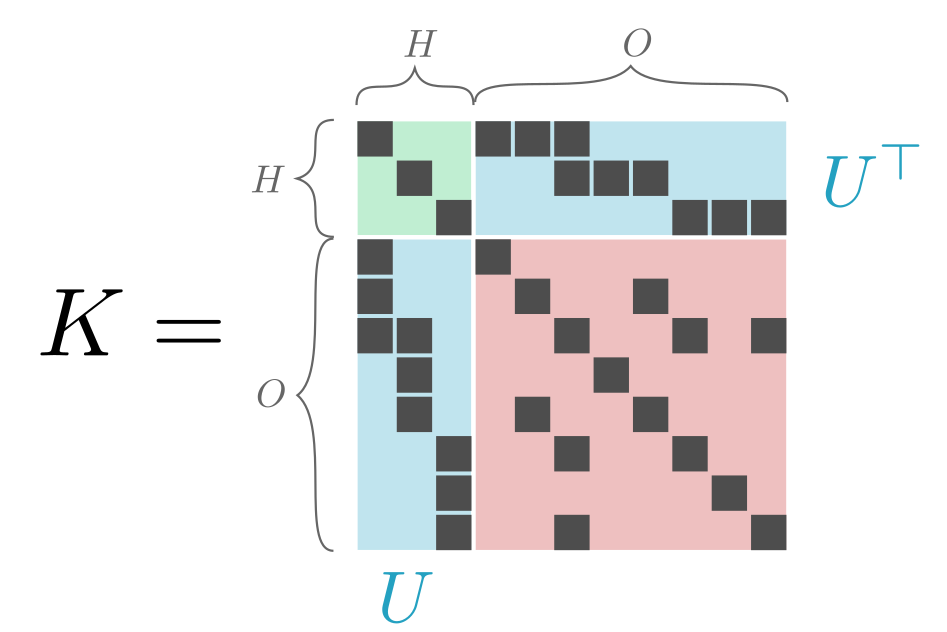
\includegraphics[width=.65\linewidth]{otherfig/matrixK.png}
  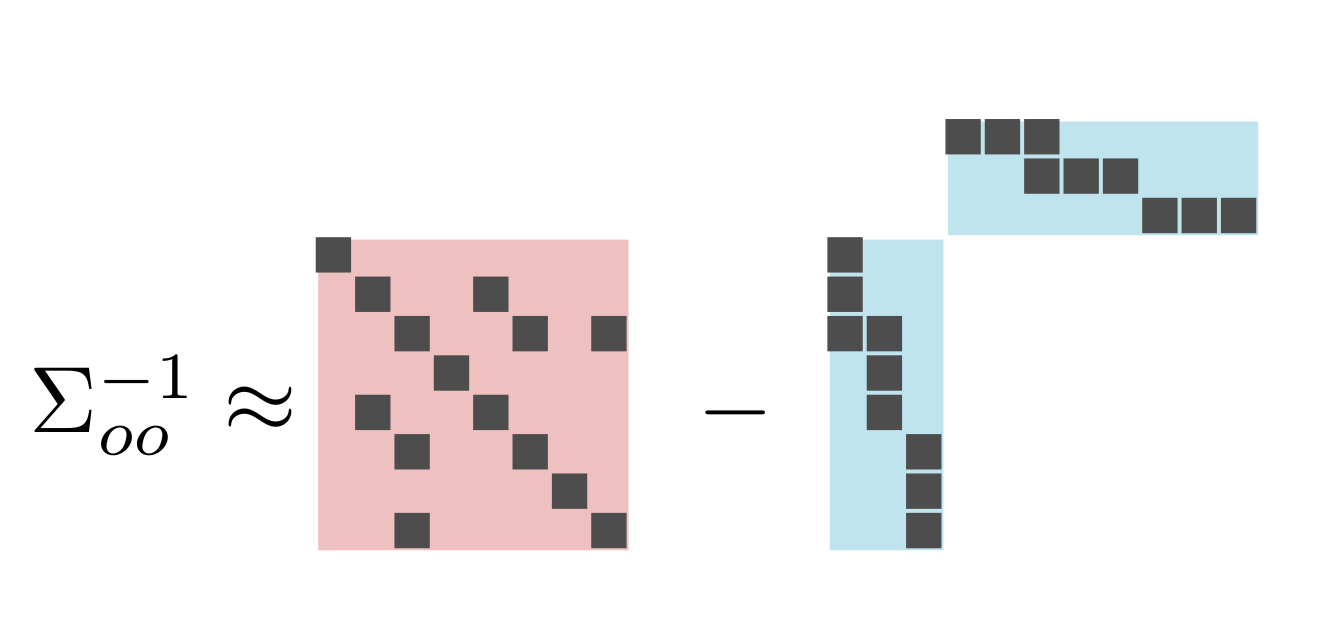
\includegraphics[width=.90\linewidth]{otherfig/matrixSigma.png}
    \caption{\TODO{ref in text}}
\end{figure}

%Since $K$ is a concentration matrix, it is positive semidefinite (p.s.d. ), which results in  $K_{OO}$ and $K_{OH}K_{HH}^{-1}K_{HO}$ being p.s.d.. $\Sigma_{OO}^{-1}$ is also p.s.d. as it is also a concentration matrix. 
\citet{chandrasekaran2010} suggest to approximate $\hat{\Sigma}$  by $S-L$ where $S$ is sparse and $L$ is low rank, with $S-L$, $S$ and $L$ p.s.d. matrices in order to ensure the statistical interpretation of the different components. The authors propose propose a convex relaxation 
%Specifically, the nonzeros of the concentration matrix correspond to the edges of the graphical model. 
%The sparsity of the complete GGM implies that $K$ is sparse. Then, $K_{OO}$ should be a sparse matrix and assuming has a small number of latent variables is low rank. \citet{chandrasekaran2010} suggest to approximate $\hat{\Sigma}$  by $S-L$ where $S$ is sparse and $L$ is low rank, and propose a convex relaxation

\begin{align}
\label{opt_tr}
&\min_{S,L} f(S-L)+\lambda\left(\gamma\|S\|_{1}+ \tr(L)\right) \\
&\quad \text{s.t.} \quad S-L \succeq 0 \quad L \succeq 0, \nonumber
\end{align}

where the function $f$ is a loss function, $\lambda$ and $\gamma$ are the regularization parameters. The positivity constraint on $S$ has been dropped since it is implied by $S-L \succeq 0$ and $L \succeq 0$. Typically, in GGM seletion $f$ is the negative log-likelihood

\begin{align}
f_{ML}(M)&:=-\log\det(M) + \tr(M\hat{\Sigma}).
\end{align}

% LATER However $\textit{logdet}$ is not smooth\footnote{does not have Lipschitz gradients} preventing us from applying efficient algorithms from the family of conditional gradient, for which there is not convergence results for this setting.
 
Two other natural losses, that have the advantage of being quadratic, are the second order Taylor expansion arount the identity matrix of the log-likelihood $f_{T}$ and the score matching loss $f_{SM}$, introduced by \citet{hyvarinen2005estimation} and used for GGM estimation in \citet{lin2016estimation},
\begin{align}
f_{T}(M)&:=\frac{1}{2}\|\hat{\Sigma}^{1/2}M\hat{\Sigma}^{1/2}-I\|_2^2\\
f_{SM}(M)&:=\frac{1}{2}\tr(M^2 \hat{\Sigma})-\tr(M).
\end{align}

\citet{chandrasekaran2010} show that under appropriate technical conditions, the regularized maximum log-likelihood formulation (\ref{opt_tr}) provides estimates $(S_{n},L_{n})$ that have the same sparsity pattern and rank than $K_{OO}$ and $K_{OH}K_{HH}^{-1}K_{HO}$. 

%\TODO{explain better}
%The obtained low rank component $L_{n}$ retrieves the latent variable subspace. However it does not recover its structure, in particular the connectivity between the variables $(X_{O}$ and $X_{H})$ cannot be recoverd since ther is not a unique decomposition of the low rank component.\\
%
%
%The low rank component writes $UU^{\top}$, where $U\in\RR^{p\times h}$. If we assume that the latent variables are independent, i.e. $K_{HH}$ is  diagonal,  unicity of the decomposition $UU^{\top}$ can be achieved by imposing more structure on the low rank component, which we discuss in the next paragraph \ref{subsec:norm}. Under appropriate identifiability conditions, discussed in section \ref{sec:id}, it allows us to retrieve the structure of the full LVGGM. In order to obtain a convex formulation we introduce a norm for low rank \textit{positive semidefinite} (p.s.d.) matrices with multiple sparse factors. 


%\TODO{explain better: trying here}

The obtained low rank component $L_{n}$ retrieves the latent variable subspace. However, in general, estimates for $K_{HH}$ and  $K_{OH}$ cannot be obtained from the estimate $L_{n}$. Therefore the connectivity between the latent variables and the connectivity between latent and observed variables cannot be recovered.\\

%from the sparse plus low-rank decomposition.

%The low  rank component writes $UU^{\top}$, where $U\in\RR^{p\times h}$, and to recover the 

With the further assumption that the latent variables are independent,  i.e. $K_{HH}$ is  diagonal,  and writing the decomposition $S-UU^{\top}$, the structure of $U$, if unique,   gives the dependence structure  between the latent and the observed variables. In general unicity of $U$ is not guaranteed. If however we assume that the part of the graph $K_{OH}$ is also sparse, i.e. each latent variable is connected to a small number of observed variables, and provided that the sparsity patterns are not the same for each latent variable (for example sources connected to disjoint subsets of observed variables), we can ensure, under technical conditions discussed in section \ref{sec:id}, that the dependency structure between latent and observed variables, i.e the sparsity pattern of.$K_{OH}$, is recovered. If $U$ is unique, we recover the dependence structure  between the latent and the observed variables. Consequently we recover the structure of the full model.

%To impose sparsity in the low rank component..

%but can be achieved by imposing more structure on the low rank component, which we discuss in the next paragraph \ref{subsec:norm}. 

%With the further assumption that the latent variables are independent,  i.e. $K_{HH}$ is  diagonal,  unicity of the decomposition $UU^{\top}$ can be achieved by imposing more structure on the low rank component, which we discuss in the next paragraph \ref{subsec:norm}. Under appropriate identifiability conditions, discussed in section \ref{sec:id}, it allows us to retrieve the structure of the full LVGGM.

Unicity of $U$ can be achieved by imposing more structure on the low rank component. More precisely we want $U$ sparse with a small number of columns so $UU^{\top}$ is low rank. For this purpose we regularize with a matrix norm  introduced by \citet{richard2014tight}, which we review in the following
section.

%and that the decomposition is unique (see section \ref{sec:id} on identifiability).  Unicity of $K_{OH}$ is achieved imposing more structure on the low rank component, which we discuss in the next paragraph.
 
%talk here about structure of $K_{OO}-K_{OH}K_{HH}^{-1}K_{HO}.$  structure $S-L$ explain\\

%and three losses ML and the two quadratic\\

%$UU$ decomposition with sparsity on columns... Transition, in order to obtain convex formulation..\\
%
%\begin{align}
%FIGURE ?
%\end{align}

%\TODO{transition}

\section{POSITIVE-RANK($k$) AND ITS RELAXATION}


\citet{richard2014tight} propose a new matrix norm that yields estimates for low-rank matrices with multiple sparse factors. In particular, these authors define a norm for p.s.d. matrices \footnote{In fact it is a gauge. For more on gauges see \citet{chandrasekaran2012convex} and references therein.}  that yields to estimates with sparse and p.s.d. factors. In this section introduce the positive-rank($k$) of a p.s.d. matrix and review its convex relaxation. We assume that the sparsity of the factors is known and fixed and discuss a generalization for factors of different sparsity levels at the end of the section.

The following definition generalizes the notion of rank for p.s.d. matrices,
\begin{mydef}
(positive-rank($k$)) For a p.s.d. matrix $Z\in\RR^{p\times p}$ and for $k>1$ we define its positive-rank($k$) as the optimal
value of the optimization problem:
\begin{align*}
&\min \|c\|_0 \\ 
&\text{s.t.} \enskip Z=\sum_{i} c_i u_i u_{i}^\top, \enskip c_i\in \RR^{+}, \enskip u_{i}\in\RR^p  :  \|u_{i}\|_0 \leq k, \|u_{i}\|_2 = 1.
\end{align*}
\end{mydef}
Note that not all p.s.d. matrices can have such a decomposition, so the positive-rank($k$) can be infinite. This is in particular the case for low-rank non sparse matrices like $11^{\top}$. 

We can derive a convex relaxation of the positive-rank($k$), the convex function $\Omega_{pos,k}$, defined as follows:
%the atomic norm%\footnote{$\Omega_{pos,k}$ is not a norm but only a gauge because the set $\{u u^\top \in\RR^p  :   \|u\|_0 \leq k, \|u\|_2 = 1\}$  is not centrally symmetric} $\Omega_{pos,k}$. The next lemma provides an explicit formulation of the dual norm
\begin{mydef}
($\Omega_{pos,k}$) For a p.s.d. matrix $Z\in\RR^{p\times p}$ 
\begin{align*}
&\Omega_{pos,k}(Z):=\min \|c\|_1 \\ 
&\text{s.t.} \enskip Z=\sum_{i} c_i u_i u_{i}^\top, \enskip 
c_i\in \RR^{+}, \enskip u_{i}\in\RR^p  :   \|u_{i}\|_0 \leq k, \|u_{i}\|_2 = 1.
\end{align*}
%Equivalently, as shown in the lemma 7 of \citet{richard2014tight},
%\begin{align}
%\Omega_{pos,k}(Z):=\inf_{Z^I, I\in\mathcal{G}^p_k} \sum_{I}\tr(Z^I) \quad \text{s.t.} \quad Z^I\succeq 0 ,\quad\supp(Z^I)\subset I\times I
%\end{align}
%%where  $\mathcal{A}_{I,\succeq}:=\{Z_I\succeq 0 ,\supp(Z_I)=I\times I\}$.
\end{mydef}

We can have $\Omega_{pos,k}(Z)=+\infty$ even when $Z$ is p.s.d., if $Z$ cannot be decomposed in $k$-sparse,  rank-1 p.s.d. factors, as it is the case for $11^{\top}$. In the next lemma we give the polar norm of $\Omega_{pos,k}$:

\begin{lemm}
\label{lem:LMO}
Let $Y\in\RR^{p\times p}$ be a symmetric matrix. The polar norm of $\Omega_{pos,k}$ writes
\begin{align}
{\Omega_{pos,k}^{\circ}}(Y)= \max_{I\in\mathcal{G}^p_k}\lambda^{+}_{max}(Y_{II}).
\end{align}
\end{lemm}

It is important to note that polar norm $\Omega_{pos,k}^{\circ}$ is NP-hard to compute. Indeed it consits of a generalization to general symmetric matrices of the rank-one sparse PCA problem for p.s.d. matrices $XX^{\top}$,
\begin{align*}
\min u^{\top}XX^{\top}u \quad s.t.  \|u\|_0 \leq k,\quad \|u\|_2 = 1
\end{align*}
which is known to be an NP-hard problem \citep{moghaddam2008sparse}. In section \ref{subsec:alg} we describe an efficient heuristic to approach this problem.

%In fact $\Omega_{pos,k}$ is an atomic gauge\footnote{$\Omega_{pos,k}$ is not a norm but only a gauge because the set $\{u u^\top \in\RR^p  :   \|u\|_0 \leq k, \|u\|_2 = 1\}$  is not centrally symmetric} associated to the atomic set $\{uu^{\top}  : \|u_{i}\|_0 \leq k, \|u_{i}\|_2 = 1\}$ and the LMO in lemma \ref{lem:LMO} is the polar gauge $\Omega^{\circ}_{pos,k}$.

%\TODO{explain a lot more}
%
%$\Omega_{pos,k}$ can be generalised for different sparsity levels as
%\begin{align}
%\Omega_{\succeq}(Z):=\inf \sum_{k,i}w_{k}c_i^k \quad \text{s.t.} \quad Z=\sum_{k,i} c_i^k u_i^k u_{i}^{k\top}, \quad c_i^k\in \RR^{+} \quad u_{i}^k\in\RR^p  :   \|u_{i}^k\|_0 \leq k, \|u_{i}^k\|_2 = 1,
%\end{align}
%where $w_{k}$ is an increasing cardinality function that penalizes each sparsity level $k$ by $w_{k}$. We illustrate this generalization in the experiments.\\
%
%\TODO{better explained here}
%$\Omega_{pos,k}$ can be generalised for different sparsity levels.

$\Omega_{pos,k}$ can be generalised for different sparsity levels. In the vector case, the norm boils down to the $k$-support norm \citep{argyriou2012sparse} and different sparsity levels are considered in the ordered weighted $\ell_1$ (OWL) norm introduced by \citet{bogdan2013statistical}. We can naturally extend this idea to the matrix counterpart $\Omega_{pos,w}$ of this norms 

\begin{align*}
& \Omega_{pos,w}(Z):=\inf \sum_{k,i}w_{k}c_i^k  \\
& \text{s.t.} \enskip Z=\sum_{k,i} c_i^k u_i^k u_{i}^{k\top},c_i^k\in \RR^{+}, u_{i}^k\in\RR^p  :   \|u_{i}^k\|_0 \leq k, \|u_{i}^k\|_2 = 1.
\end{align*}
where $w_{k}$ is an increasing cardinality function that penalizes each sparsity level $k$ by $w_{k}$. We illustrate this generalization in the experiments.


%1) normes liees a la k-support norm\\
%2) autres tailles considerees dans le cas vectoriel OWL \citet{bogdan2013statistical}
%3) et que on peut naturellement ... the matrix counterpart of this norms. A la condition que les poids soient decroissants.



\section{CONVEX FORMULATION}
%Let $(x_1,..,x_n)$ be $n$ samples of dimension $p$ and   $\hat{\Sigma}$ the empirical covariance. A natural way to approximate a given sample covariance matrix by a model which the concentration matrix decomposes into a sparse and $k$-low-rank matrix is a regularized using $\ell_1$ norm for recovering sparse component and the convex relaxation of $k$-rank for recovering the $k$-low-rank component. Hence we consider the following convex optimization problem
%\begin{align}
%\label{opt}
%\min_{S,L} f(S-L)+\mu\|S\|_{1}+\lambda\Omega_k(L) \quad s.t. \quad S-L \succeq 0 \quad L \succeq 0,
%\end{align}
%where  $f$ represents the loss function.
% Typically,in Graphical model seletion $f$ is the log-likelihood, as proposed in \citet{chandrasekaran2010}. However \textit{logdet} is not Lipschitz preventing us from applying efficient algorithms of the family of conditional gradient, for which there is not convergence results for this setting.  Two other natural losses, which have the advantage of being quadratic, are the second order taylor expansion of the log-likelihood $f_{T}$ and the score matching loss $f_{SM}$, introduced by \citet{hyvarinen2005estimation} and used for graphical model estimation in \citet{lin2016estimation}.
%\begin{align}
%f_{SM}(K)&:=\frac{1}{2}\tr(K^2 \hat{\Sigma})-\tr(K) \\
%f_{T}(K)&:=\frac{1}{2}\|\hat{\Sigma}^{1/2}K\hat{\Sigma}^{1/2}-I\|_2^2.
%\end{align}

We use $\Omega_{pos,k}$ to impose structure on the low rank component and consider the following convex optimization problem,
\begin{align}
\label{opt}
\min_{S,L} f(S-L)+\lambda\big(\gamma\|S\|_{1}+\Omega_{pos,k}(L)\big) \quad s.t. \quad S-L \succeq 0 
\end{align}
Note that the nonnegativity constraint on $L$ is no longer necessary since the norm $\Omega_{pos,k}$ only provides symmetric p.s.d. matrices, as a sum of p.s.d. rank-one matrices.
%Since the norm $\Omega_k$ only provides symmetric p.s.d. matrices, as a sum of p.s.d. rank-one matrices, the nonnegativity constraint on $L$ is no longer necessary and can be dropped. 
\TODO{say that we drop constraint $ S-L \succeq 0 $}
\begin{align}
\label{opt_nc}
\min_{S,L} f(S-L)+\lambda\big(\gamma\|S\|_{1}+\Omega_{pos,k}(L)\big)
\end{align}
%\begin{rem} 
%The regularization $\gamma\|S\|_{1}+\Omega_k(L)$ defines an atomic norm on matrices. $\bar{\Omega}(M):=\inf\{\gamma\|A\|_{1}+\Omega_k(B)\mid M=A+B\}$ is an atomic norm and its polar norm is given by 
%\begin{align*}
%{\bar{\Omega}^{\circ}}(Y)=\max\left(\frac{\|Y\|_{\infty}}{\gamma},\Omega_{pos,k}^{\circ}(Y)\right).
%\end{align*}
%\end{rem}
%
%In order to rewrite our problem as a simple convex regularized by $\bar{\Omega}$, we drop the nonegativity constraint on $S-L$. Thus our problem is rewritten as
%\begin{align}
%\label{opt_at}
%\min_{M} f(M)+ \bar{\Omega}(M) \quad s.t. \quad M \succeq 0,
%\end{align}
%and $M$ writes as a sum of atoms of $\ell_1$ and atoms of $\Omega_k$. Therefore we can recover a sparse component and a low-rank component with multiple sparse factors.\\

\section{ALGORITHM}

We apply an alternate optimization approach. The procedure is explained in algorithm \ref{alg:alt} and: first we update $S$ by optimizing problem (\ref{opt_nc}) with $L$ fixed, then we update $L$ by solving problem (\ref{opt_nc}) with $S$ fixed. To optimize the sparse factor $S$ we use FISTA algorithm \citep{beck2009fast}. For optimizing the low rank factor we apply an efficient algorithm for quadratic losses recently proposed by \citet{vinyes2017}(\texttt{FCG}). Therefore we choose to consider quadratic losses $f_{T}$ and $f_{SM}$, introduced in section \ref{sec:ggm} in order to obtain an efficient algorithm.\\

The \texttt{FCG} algorithm consists of applying a Fully Corrective Frank Wolfe \citep{LacosteFCFW} to a regularized optimization problem. We briefly review Frank Wolfe (FW) algorithm \citep{frank1956algorithm}. FW algorithm, also known as conditional gradient, is particularly well suited for constrained quadratic optimization of the form
\begin{align*}
\min f(x) \quad s.t. \quad x\in \mathcal{C}
\end{align*}
where $\mathcal{C}$ is convex and bounded. In particular $\mathcal{C}$ can be the convex hull of a set of atoms $\A$  In each iteration FW needs to solve a linear minimization oracle (LMO) which solves the optimization problem
\begin{align}
\rm{{LMO}}_{\mathcal{C}}(y) := \arg\min_{z \in \mathcal{C}} \left\langle y,z \right\rangle.
\end{align}
At each iteration FW selects a new atom $a^t$ from $\mathcal{C}$ querying the LMO and computes the new iterate as a convex combination of $a^t$ and the old iterate $x^t$. The convex update can be done by line search. Another variant, called the fully corrective FW (FCFW), is discussed in \citet{LacosteFCFW}. FCFW consits of finding the convex combination of all previously selected atoms $(a^i)_{i<t}$. The algorithm can be generalized for regularized problems. \texttt{FCG} algorithm consists of applying a FCFW, for which we need to compute the following LMO 
\begin{align}
% \rm{{LMO}}_{\mathcal{C}}(y) := \arg\min_{z \in \mathcal{C}} \left\langle y,z \right\rangle.
\rm{{LMO}}_{\Omega_{pos,k}}(M) :={\arg\max}_{\|u\|_0=k, \|u\|_ 2=1 } u^{\top}Mu,
% &=\max_{I\in\mathcal{G}^p_k}\lambda^{+}_{max}(Y_{II})
\end{align}
at each iteration, and subsequently use a working set algorithm to solve the fully corrective step.\\

We propose to use a Truncated Power Iteration (TPI) heuristic introduced by \citet{yuan2013truncated} to approximate the oracle. TPI is suited for p.s.d. matrices. In order to apply the TPI to general symmetric matrices, we add the frobenius norm of the matrix before applying it. \\

%The procedure is explained in algorithm \ref{alg:colgen_ggm} and consists on three loops: first we augment the atomic set $\mathcal{A}^{t}$ for atoms of  $\Omega_{pos,k}$, then we solve the subproblem (\ref{opt_ps}) with \texttt{FCG} that internally uses an active-set procedure.


\begin{algorithm*}
\caption{Alternate minimization}
\label{alg:alt}
\begin{algorithmic}[1]
\State\textbf{Require: } $f$ quadratic, tolerance $\epsilon$ , maximum iterations $T$
\State\textbf{Initialization: } $S^{0}=0$, $L^{0}=0$, $t=0$
\For{$t=1..T$}
\State Compute $S^{t}$ applying \texttt{FISTA} on problem (\ref{opt_nc}) with $L^{t-1}$ fixed
\State Compute $L^{t}$ applying \texttt{FCG} on problem (\ref{opt_nc}) with $S^{t}$ fixed
\State Compute $udg$ upper bound on global duality gap
\If {$udg < \epsilon$}
\State return $S^{t}, L^{t}$
\EndIf
\EndFor
\end{algorithmic}
\end{algorithm*}





\section{IDENTIFIABILITY CONDITIONS}

\TODO{We proove identifiability on a restricted setting. Proof of sufficient conditions for exact recovery of the components by solving optimization problem \ref{opt_nc} is out of scope of this paper.}\\
We aim to introduce sufficient conditions such that $(S^*, L^*)$ is an optimum of the problem
$$
\displaystyle \min \gamma \|S\|_1+\Omega_{k,\succeq}(L) \quad \text{\st} \quad M=S+L
$$

Setting for $S^*$ and $L^*:=\sum_{I_i \in \mathcal{I}} L^{I_i}$. $I$ are disjoint and $L^{I_i}:=s_i u^i {u^i}^{\top}$ where $supp(u^i)\subset I_i$.

Define tangent spaces $\T_s$ and $\T_I$. We consider several type of subspaces
$$\bar{\T}_I:=\{M \in \RR^{p \times p}\mid  M=M^\top, \: \supp(M)\subset I \times I\},$$
$$\T_I(U):=\{M \in \bar{\T}_I\mid \: M=UX^\top+XU^\top,\: X \in \RR^{\text{rank}(U) \times p} \},$$
Let $\T^c_I(U)$ denote the orthogonal complement\footnote{Note in particular that it is not the orthogonal complement in the entire space.} of $\T_I(U)$ in $\bar{\T}_I$. 
$$\T(U):=\T_{[\![p]\!]}(U)$$
$$\T_s(A)=\{M \in \RR^{p \times p}\mid  \: M=M^\top, \: \supp(M)\subset \supp(A)\}.$$
The projections on the corresponding subspaces are $\mathcal{P}_{\T_s(A)}(M)=M_S$ and $\mathcal{P}_{\T_I(U)}(M)=\mathcal{P}_{U}(M_{II})$ with $$\mathcal{P}_U(M):=M-(I-UU^\top)M(I-UU^\top).$$


For the unicity of the decomposition tangent spaces must intersect transversally, that is that the collection of subspaces $\T_i$ are linearly independent in the sense that for any $i$, $\T_i \cap \text{span}(\T_j)_{j \neq i}=\{0\}$.


\begin{assumption}The degree of the sparse part of the graph is bounded by $k_0$, i.e. $\forall i\in\itgset{p}$,  $\|S^*_i.\|\leq k_0$ .
\end{assumption}

\begin{assumption}The entries of $u^i$ are bounded, i.e. $\forall j\in I_i$,  $\underline{\tau} / k \leq (u_j^i)^2 \leq \bar{\tau} / k$.
\end{assumption}

$(S^*, L^*)$ is an optimum if an only if there exists a dual $Q$ satisfying first order optimality conditions

\begin{align*}
Q\in \gamma \partial \|.\|_1(S^*) \quad \text{and} \quad Q\in \partial \Omega_{pos,k}(.)(L^*)
\end{align*}

Characterization of subgradients $\ell_1$ and $\Omega_{pos,k}$, introduce the projections on the tangent subspaces.

\begin{lemma}(characterization of $\ell_1$ subgradient) $Q\in \gamma \partial \|.\|_1(S^*)$ if and only if
\item[(i)] $\mathcal{P}_{\T_s(S^*)}(Q)=\gamma sign(S^*)$
\item[(ii)] $\|Q_{S^c}\|_{\infty}<\gamma$
\end{lemma}
\begin{proof}
By the characterization of the subgradient of a norm we have $Q\in \gamma \partial \|.\|_1(S^*)$ if and only if
\begin{align}
\|Q\|_{\infty}\leq \gamma \quad \text{and} \quad \left\langle Q,S^*\right\rangle=\gamma\|S^*\|_1. \label{eq:subgl1}
\end{align}
Let us decompose $Q$ on $\T_s(S^*)$ and the corresponding orthogonal space $\T_s(S^*)^{\perp}$, $Q= Q_S+Q_{S^c}$. Since $S^*\in\T_s(S^*)$, we have $\left\langle Q_S,S^*\right\rangle=\gamma\|S^*\|_1$, that rewrites as  $\left\langle Q_S-\gamma sign(S^*),S^*\right\rangle=0$ and gives $Q_S=\gamma sign(S^*)$.\\
On the other hand 
$$\|Q_S+Q_{S^c}\|_{\infty}=\max\left(\|Q_S\|_{\infty},\|Q_S\|_{\infty}\right)=\max\left(\gamma,\|Q_S^c\|_{\infty}\right).$$
\end{proof}
\begin{lemma}(characterization of $\Omega_{pos,k}$ subgradient) $Q\in \partial \Omega_{pos,k}(.)(L^*)$ if and only if
\item[(i)] for all $I \in \I,\:\mathcal{P}_{\T_I(\uI)}(Q)=\uI{\uI}^\top$
\item[(ii)] for all $I \in \I,\:\lambda_{\max}^+\big (\mathcal(P)_{\T_I^c(\uI)}(Q) \big )<1$
\item[(iii)] for all $J \in \mathcal{G}^p_k \backslash \I, \: \lambda_{\max}^+(Q_{JJ})\leq 1$
\end{lemma}
\begin{proof}
By the characterization of the subgradient of a gauge we have  $Q\in \partial \Omega_{pos,k}(.)(L^*)$ if and only if
\begin{align}
\lambda_{\max}^+(Q)\leq 1\quad \text{and} \quad \left\langle Q,L^*\right\rangle=\Omega_{pos,k}(L^*). \label{eq:subgom}
\end{align}
Note that the inequality implies that $u^{\top}Qv\leq1$ for any unit vectors $u,v$. By definition of $L^*$, the equality becomes $\sum_{I_i\in\mathcal{I}}s_i ({u^i}^{\top}Qu^i-1)=0$. Since all terms of the sum are non negative we must have ${u^i}^{\top}Qu^i=1$. Using the fact that $u^i$ have distinct supports, we have that $Q$'s maximum eigenvalue is 1, associated to eigenvector $u^i$ and we can write $Q=u^i{u^i}^{\top} + W_i$ with $W_i$ orthogonal to the space of matrices with column-space spanned by $u^i$. More specifically, if we restrict ourselves to subspace $I_i\times\I_i$, $Q_{I_iI_i}$ is uniquely decomposed on $\T_{I_i}\bigoplus \T_{I_i^c}$. The equality condition of \ref{eq:subgom} becomes $(i)$.\\ On the other hand,
\begin{align*}
\lambda_{\max}^+(Q_{I_iI_i})
&=\max_{\substack{v: \|v\|\leq 1\\ supp(v)\in I_i }}v^{\top}\left(u^i{u^i}^{\top} + \mathcal(P)_{\T_I^c(u^i)}(Q) \right)v \\
&=\max(1,\lambda_{\max}^+\big (\mathcal(P)_{\T_I^c(u^i)}(Q) \big ),
\end{align*}
where the last inequality \TODO{orthogonal spaces}.
Finally,
\begin{align*}
&\lambda_{\max}^+(Q) = \max_{\substack{v: \|v\|\leq 1\\ v\in \mathcal{G}^p_k }}v^{\top}Qv\\
&= \max \left( \max_{I_i\in \I}\lambda_{\max}^+(Q_{I_iI_i}), \max_{J \in \mathcal{G}^p_k \backslash \I} \lambda_{\max}^+(Q_{JJ})\right)
\end{align*}
which results in conditions $(ii)$ and $(iii)$.
\end{proof}

\TODO{From identifiability theory chapter Low rank with sparse factors + sparse decomposition.. Check notations and reformulate if necessary. }\\

Let 
\begin{eqnarray*}
\xxi(\T_s(S),\T_J(V))&=&\max \{ {\|M_S\|_\infty} \mid M \in \T_J(V), \: \|M\|_{\op}\leq 1\}\\
\xxi(\T_I(U),\T_s(S))&=&\max \{ {\|\mathcal{P}_{U}(M_{II})\|_{\op}} \mid M \in \T_s(S), \: \|M\|_{\infty}\leq 1\}\\
\xxi(\T_I(U),\T_J(V))&=&\max \{ {\|\mathcal{P}_{U}(M_{II})\|_{\op}} \mid  M \in \T_J(V), \: \|M\|_{\op}\leq 1\}\\
\xi(\T_J(V))&=&\max \{ {\|M\|_\infty} \mid M \in \T_J(V), \: \|M\|_{\op}\leq 1\}\\
\mu_I(\T_s(S))&=&\max \{ {\|M_{II}\|_\op} \mid M \in \T_s(S), \: \|M\|_{\infty}\leq 1\}\\
\end{eqnarray*}

\begin{theorem}
\label{theo:two}
If $M^*=S^*-L^*$ with $L^*=\sum_{I \in \mathcal{I}} L^{\sss{I}}$, $\supp(L^{\sss{I}}) \subset I \times I$ for $\I \subset \mathcal{G}^p_k$ %(where $\mathcal{G}^p_k$ is the collection of all subsets of size $k$ of $[\![p]\!]$) 
and $L^{\sss{I}}=U^{\sss{I}} D^{\sss{I}} {U^{\sss{I}}}^\top$ the eigenvalue decomposition of $L^{\sss{I}}$.
Let $\mu'_I=\xxi(\T_I(U),\T_s(S))$, $\xi'_I :=\xxi(\T_s(S),\T_I(U))$, $\mu_I:=\mu_I(\T_s(S))$, $\xi_I:=\xi(\T_I(U))$, 
$$\alpha_I:=\frac{1-\mu'_I\xi'_I}{1+\max(\gamma \mu'_I,\frac{1}{\gamma} \xi'_I)} \qquad \text{and} \qquad \epsilon_I :=\max \big (\|\mathcal{P}_{\T_I(\uI)}(\gamma \text{sign}(S^*))\|_{\op}, \gamma^{-1}\|\uI {\uI}^\top\|_{\infty} \big ).$$

Assume that for all $(I,I') \in \I \times \I, I \cap I'=\varnothing$. If $$\displaystyle\max_{I \in \I} \max(\mu_I,\xi_I) (1+\frac{\epsilon_I}{\alpha_I})<1, \quad \displaystyle \max_{J \in \mathcal{G}^p_k} \lambda_{\max}^+\big (S^*_{\bar{I}^c \cap (J \times J)} \big ) <1$$ %\quad  
%\text{and}  \quad \max_{J \in \mathcal{G}^p_k, J \neq I}\lambda_{\max}^+(\uI_J{\uI_J}^\top)<1,$$ 
with $\displaystyle \bar{I}=\bigcup_{I \in \I} I \times I$,
then the solution of the optimization problem $$\displaystyle \min \gamma \|S\|_1+\Omega_{k,\succeq}(L) \quad \text{\st} \quad M=S+L$$
 the decomposition given by $\big (S^*,(D^{\sss{I}} \big)_{I \in \I},(\uI)_{I \in \I} \big )$ as a solution.
\end{theorem}
\begin{proof}
We follow the general proof scheme of \citet{chandrasekaran2011rank}. The optimization problem admits the unique announced solution if it satisfies first order gradient condition in the sense that there exists a subgradient $Q \in \RR^{p \times p}$ that satisfies the following conditions
\BET
\item[(i)] for all any $M^\sss{s} \in \T_s(S^*)$ and $(M^{\sss{I}})_{I \in \I}$ with $M^{\sss{I}} \in \T_I(\uI)$, $M^\sss{s}+\sum_{I \in \I} M^{\sss{I}}=0 \: \Rightarrow \: (M^{\sss{I}}=0, \:I \in \I)$.
\item[(ii)] for all $I \in \I,\:\mathcal{P}_{\T_I(\uI)}(Q)=\uI{\uI}^\top$
\item[(iii)] $\mathcal{P}_{\T_s(S^*)}(Q)=\gamma sign(S^*)$
\item[(iv)] for all $I \in \I,\:\lambda_{\max}^+\big (\mathcal(P)_{\T_I^c(\uI)}(Q) \big )<1$
\item[(v)] $\|Q_{S^c}\|_{\infty}<\gamma$
\item[(vi)] for all $J \in \mathcal{G}^p_k \backslash \I, \: \lambda_{\max}^+(Q_{JJ})\leq 1$
\EET
We now prove the different statements. As a consequence of the assumption that $I \cap I'=\varnothing, (I,I') \in \I \times \I,$ the space of symmetric squared matrices can be written as the direct sum of the spaces $(\bar{\T}_I)_{I \in \I}$ and of the space $\T^c:=\{M \in \RR^{p \times p} \mid  M=M^\top, \: M_{\bar{I}}=0\}$. Which entails that part of the properties to prove can be shown independently on the elements of the direct sum, namely the four first properties. 
\BET
\item[(i)] Since $I \cap I'=\varnothing,\: I\neq I'$, we can have $M^\sss{s}+\sum_{I \in \I} M^{\sss{I}}=0$ if and only if $M^\sss{s}_{II}+ M^{\sss{I}}_{II}=0$ for all $I$ and $M^\sss{s}_{\bar{I}}=0$. But if $M^\sss{s}_{II}+ M^{\sss{I}}_{II}=0$ using the argument of \citet{chandrasekaran2011rank} or Lemma~\ref{lem:zero_inter} for two subspaces, we have that $M^\sss{s}_{II}= M^{\sss{I}}_{II}=0$ which shows the result.
\item[(ii)], (iii), (iv) and (v) The existence and the uniqueness of a $Q$ follow from the application of Theorem~\ref{theo:two} to each of the subspaces $(\T_I)_{I \in\I}$ and $\T^c$ separately. The theorem also proves directly that (iii),(iv) and (v) hold.
\item[(iv)] For any $J$ such that $(J \times J) \cap \bar{I}=\varnothing,$ the fact that $\lambda_{\max}^+(Q_{JJ})<1$ follows directly from the fact that then $Q_{JJ}=S^*_{JJ}$ and that $\lambda_{\max}^+(S^*_{(J \times J) \cap \bar{I}^c})<1$.
If $(J \times J) \cap \bar{I} \neq \varnothing$ then let $\mathcal{I}_{J}$ be the collection of sets in $\I$ such that $J$ and $I$ intersect. Note that since these elements $I$ are disjoint $\bar{\T}_J$ is the direct sum of the $(\bar{\T}_{J\cap I})_{I \in \I_{J}}$ and of their orthogonal complement in $\bar{\T}_J$.
As a consequence
$$\lambda_{\max}^+(Q_{JJ}) \leq \Big ( \lambda_{\max}^+(Q_{(J \times J) \cap \bar{I}^c}) \Big ) \vee \max_{I \in \I_{J}} \lambda_{\max}^+(Q_{(J\cap I) \times (J \cap I)}).$$
But $\lambda_{\max}^+(Q_{(J \times J) \cap \bar{I}^c}) <1$ as before and 
we need to show that $\lambda_{\max}^+(Q_{(J\cap I) \times (J \cap I)}) \leq 1.$
%Since $Q_{(J\cap I) \times (J \cap I)=\uI_J\uI_J$
\EET
\end{proof}

Consider a set of indices $J$, which will be fixed throughout this section\footnote{Although most of the variables defined in this section depend on $J$, we do not make this dependence explicit to lighten notations.}.

Denote $u_i:=u_{I_i}$, $\check{u}_i=u^{I_i}_J$ and $v_i:=\frac{\check{u}_i}{\|\check{u}_i\|}$. Let $\kappa:=|\{i \mid I_i \cap J \neq \varnothing\}|.$ Let $k_i:=|I_i \cap J|$. Since, we assume that all the entries of $u_i$ are in the interval $[\underline{\tau}, \overline{\tau}]$, note that we have $k_i \underline{\tau} k_i \leq (\check{u}_i^\top v_i)^2 \leq k_i \overline{\tau}$.

Let $V_i^c \in \RR^{p \times k-1}$ be such that $[v_i, V_i^c]$ forms an orthonormal basis of $\text{span}(e_j)_{j \in J \cap I_i}$. 

Let $V:=[v_1,\ldots,v_\kappa] \in \RR^{k \times \kappa}$ and $V^c:=[V_1^c,\ldots, V^c_\kappa] \in \RR^{k \times   (k-1) \kappa}$. 

By construction, $[V,V^c]$ is an orthonormal basis of $\text{span}(e_j)_{j \in J}$.
Then we have $Q_{JJ}=[V,V^c] \check{Q}_{JJ} [V,V^c]^\top$ with

$$\check{Q}_{JJ}=
\begin{bmatrix}
V^\top Q V & V^\top Q V^c\\
{V^c}^\top Q V & {V^c}^\top Q V^c\\
\end{bmatrix}
$$

We have $[V^\top Q V]_{ii}=v_i^\top Q v_i=v_i^\top [u_i u_i^\top+R_i] v_i$
with $R_i=\mathcal{P}_{\mathcal{T}^{\bot}_{I_i}(u_i)}=(I-u_i u_i^\top)\, Q_{I_iI_i}\,  (I-u_i u_i^\top).$

We have on the one hand, $v_i^\top u_i u_i^\top v_i=(\check{u}_i^\top v_i)^2 \leq k_i \overline{\tau}^2$. On the other, if $\check{v}_i:=(I-u_iu_i^\top) v_i$ then 
$$v_i^\top R_i v_i=(u_i u_i^\top v_i +\check{v}_i)^\top R_i (u_i u_i^\top v_i +\check{v}_i)=\check{v}_i^\top R_i \, \check{v}_i \leq \|R_i\|_{\op} \, \|\check{v}_i\|^2_2 \leq (1-k_i\underline{\tau}^2) \|R_i\|_{\op}$$

So finally, since $\|R_i\|_{\op} \leq \|\gamma sign(S_{I_iI_i})+\varepsilon^{s_i}\|_{\op} \leq \xi_i (1+\frac{\epsilon}{\alpha}),$ we have 
$$v_i^\top Q v_i \leq k_i \overline{\tau}^2+(1-k_i\underline{\tau}^2) \xi_i (1+\epsilon/\alpha).$$
 
 
Then for $[V Q V^c]$, the fact that $v_i$ is proportional to the projection of $u_i$ on ${\rm span}(e_j)_{j \in J}$, we have $u_i^\top V^c=0$ so that

$$\|v_i^\top Q V_i^c\|_{\op}=\|v_i^\top R_i V_i^c\|_{\op} \leq \|v_i^\top R_i\|_{2}.$$
 
\begin{lemma}
If $u$ is a vector such that $\|u\|_2=1$, then we have
 $\|u^\top Z\|_{2} \leq \|\mathcal{P}_{\mathcal{T}(u)}\|_{\op}  \leq 2\, \|u^\top Z\|_{2}.$
\end{lemma}
\begin{proof}
We use the following key identity
 
 $$\mathcal{P}_{\mathcal{T}(u)} u=(uu^\top Z + Z uu^\top - u u^\top Z u u^\top) u =Zu$$

$$\|\mathcal{P}_{\mathcal{T}(u)}\|_{\op} \geq \|u^\top \mathcal{P}_{\mathcal{T}(u)}\|_{2} \geq \|u^\top (uu^\top Z + Z uu^\top - u u^\top Z u u^\top) \|_{2}=\|u^\top Z\|_{2}
$$
\begin{eqnarray*}
\|\mathcal{P}_{\mathcal{T}(u)}\|_{\op}:=\|uu^\top Z + Z uu^\top - u u^\top Z u u^\top\|_{\op}  
& \leq & \, \|uu^\top Z\|_{\op} + \|Z uu^\top - u u^\top Z u u^\top\|_{\op}\\
& \leq &  \, \|u^\top Z\|_{2} + \|Z uu^\top - u^\top Z u u^\top\|_{2}\\
& \leq &  \,\|u^\top Z\|_{2} + \sqrt{u^\top Z^2 u - u^\top Z u }\\
& \leq & 2 \, \|u^\top Z\|_{2}
\end{eqnarray*}
\end{proof}

To summarize

$$\check{v}_i^\top Q \check{v}_j=v_i^\top u_i u_i^\top [Q_{S}]_{I_i I_j} u_j u_j^\top v_j$$

%$u_i^\top Z u_j$

$$|u_i^\top Z u_j| = |u_i \mathcal{P}_{\mathcal{T}(u_j)}(Z) u_j^\top|=|u_i \mathcal{P}_{\mathcal{T}(u_i)} \circ \mathcal{P}_{\mathcal{T}(u_j)}(Z) u_j^\top| \leq \|\mathcal{P}_{\mathcal{T}(u_i)} \circ \mathcal{P}_{\mathcal{T}(u_j)}(Z)\|_{\op} \leq \xi_{ij} \|\mathcal{P}_{\mathcal{T}(u_j)}(Z)\|_{\op} \leq \zeta_{ij} \zeta_{js}.$$

We can use similar ideas to bound:
\begin{itemize}
\item $\check{v}_i^\top Q \check{v}_j$ 
\item $v_i^\top Q v_j$
\item $\|v_i^\top Q V_j^c\|_2$
\end{itemize}

\section{EXPERIMENTS}
\label{experiments}
\subsection{Toy examples}

We consider three differents LVGGM with $p=45$ observed variables, with a tree structure on observed variables and the following structure on latent variables :
\begin{itemize}
\item \textit{model 1}: consists of $h=3$ latent variables, we split observed variables in three groups of size $15$ and connect each group to a single latent variable.
\item \textit{model 2}: consists of $h=3$ latents variables we split observed variables in three groups of different sizes ($20,15$ and $10$) and connect each group to a single latent variable.
\item \textit{model 3}: consists of of $h=4$ latent variables. We select $4$ overlapping groups of size $15$ of observed variables, with a $0.26$ overlap, and connect each one of them to a different latent variable.
\end{itemize}

%- \textit{model 1}: consists of $h=3$ latent variables, we split observed variables in three groups of size $15$ and connect each group to a single latent variable.\\
%- \textit{model 2}: consists of $h=3$ latents variables we split observed variables in three groups of different sizes ($20,15$ and $10$) and connect each group to a single latent variable.\\
%- \textit{model 3}: consists of of $h=4$ latent variables. We select $4$ overlapping groups of size $15$ of observed variables, with a $0.26$ overlap, and connect each one of them to a different latent variable.\\

We generate $50\times p$ samples for each model. Figure \ref{fig:synth} shows the estimated complete concentration matrix obtained for our formulation with the score matching loss compared to a regularization $\ell_1+\tr$, as in \citet{chandrasekaran2010}. For  the $\ell_1+\tr$ regularization we perform an SVD on the obtained low rank matrix to visualize the effect of latent variables. For the first two models the size of the blocks is fixed and for the third model we use the extention of the introduced matrix norm $\Omega_{k,\succeq}$ where the blocks can have different sizes, see section \ref{subsec:norm},  and each size $k$ is penalized by $w_{k}=\sqrt{k}$, see section \ref{subsec:norm}. The regularization parameters are chosen so to recover the desired sparsity pattern for the sparse component and rank for the low rank component.  The decomposition of the low rank component for $\ell_1+\tr$ regularization is not unique so this method cannot recover the effect of latent variables. Both methods recover the sparsity pattern of $S$ and only our methods recovers the structure of the effects of latent variables.

%\begin{figure}[h]
%  \begin{minipage}[ccc]{\linewidth}
%  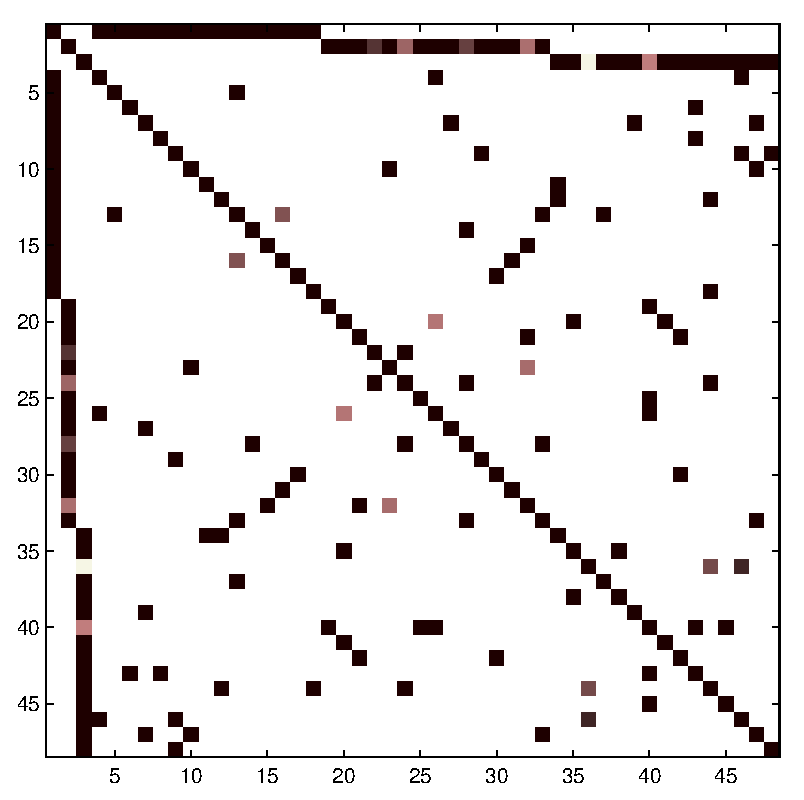
\includegraphics[width=3cm]{fig/disjoint_om}
%  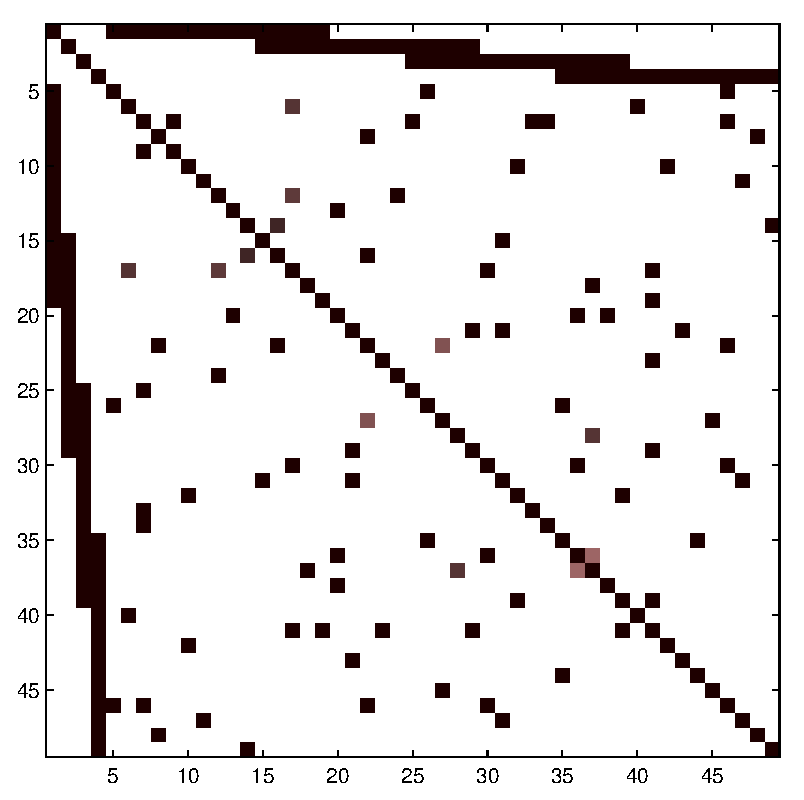
\includegraphics[width=3cm]{fig/overlap_om}
%  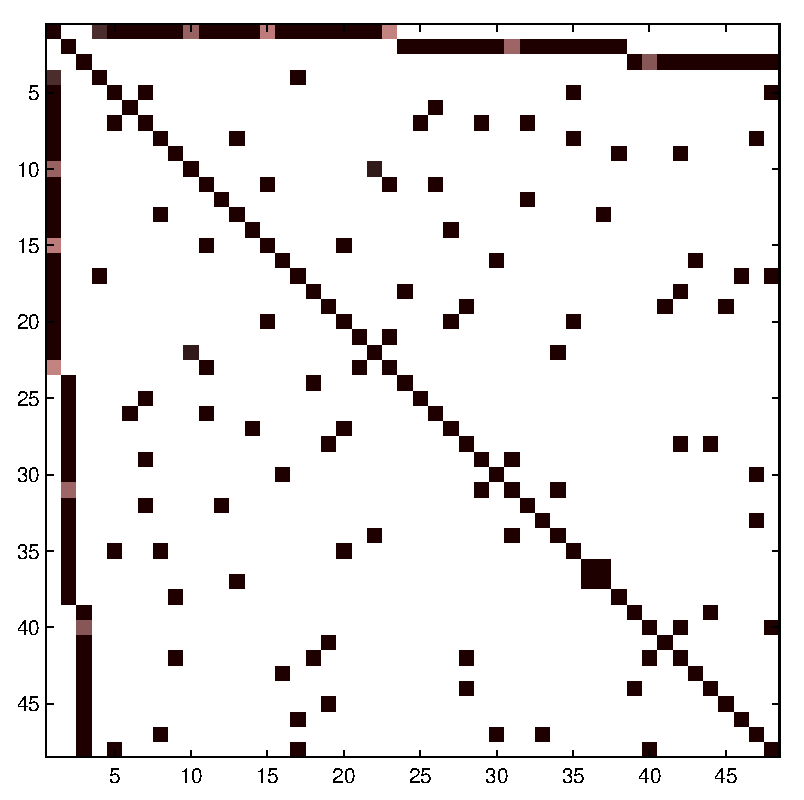
\includegraphics[width=3cm]{fig/diff_om}
%  \end{minipage}
%  \begin{minipage}[ccc]{\linewidth}
%  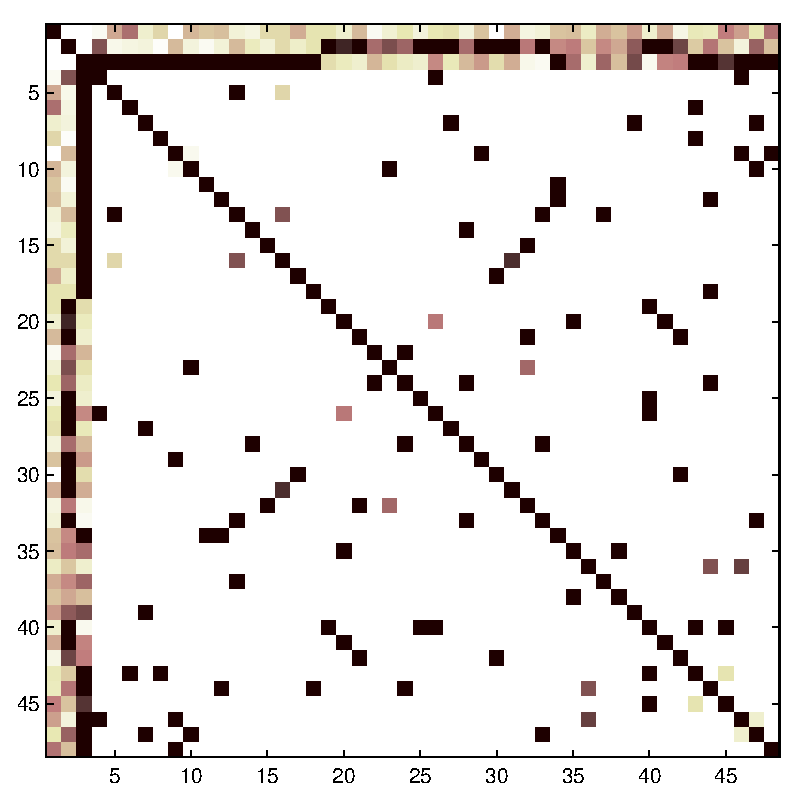
\includegraphics[width=3cm]{fig/disjoint_tr}
%  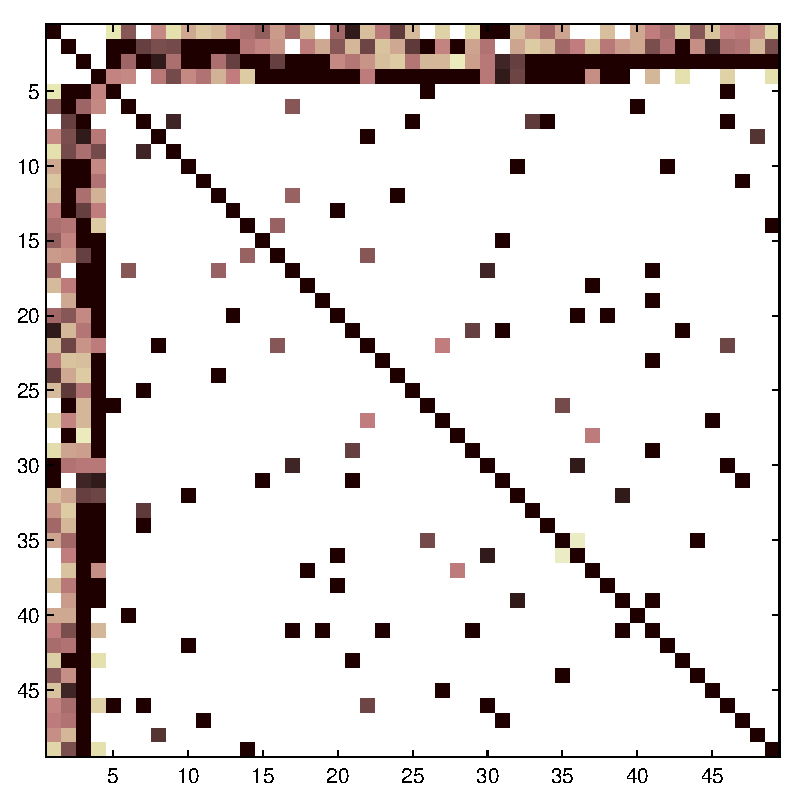
\includegraphics[width=3cm]{fig/overlap_tr}
%  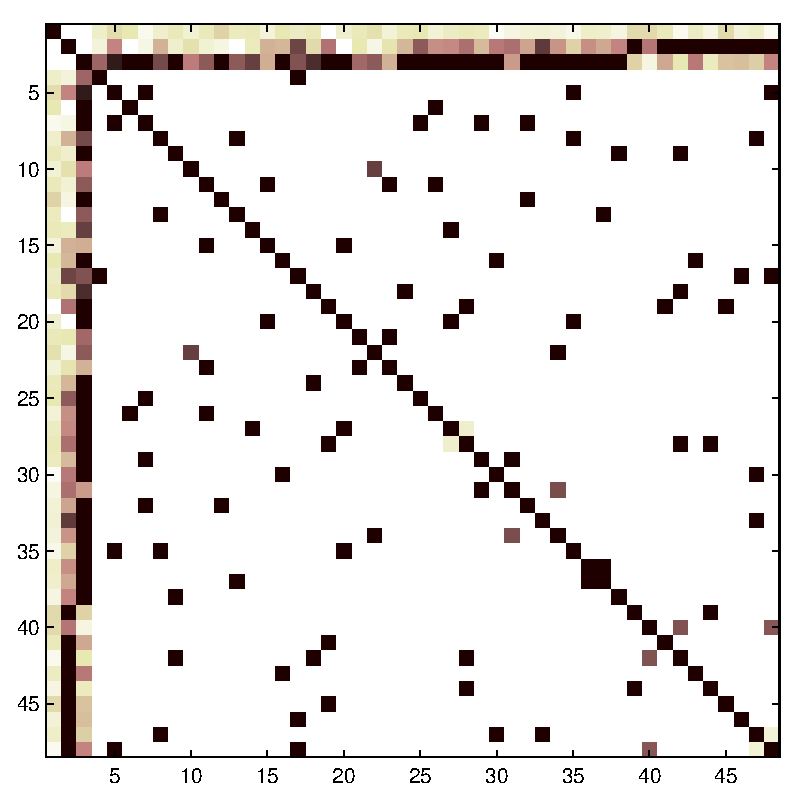
\includegraphics[width=3cm]{fig/diff_tr}
%  \end{minipage}
%  \caption{Experiment for the $k$-chain group Lasso. Top:number of pivots, i.e., drop/full step in active set. Left figure shows the number of pivots per active set call and right plot shows the total number of pivots during iterations. Bottom: evolution of the number of active atoms in our algorithm.}
%\end{figure}

%\begin{figure}
%\center
%\hfill
%\subfigure[Title A]{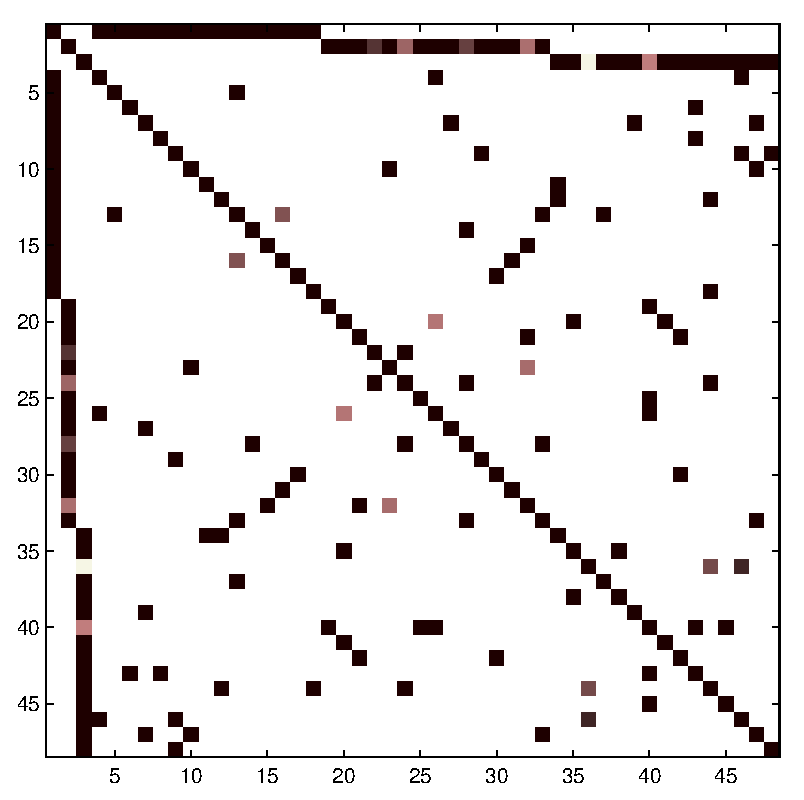
\includegraphics[width=3cm]{fig/disjoint_om}}
%\hfill
%\subfigure[Title B]{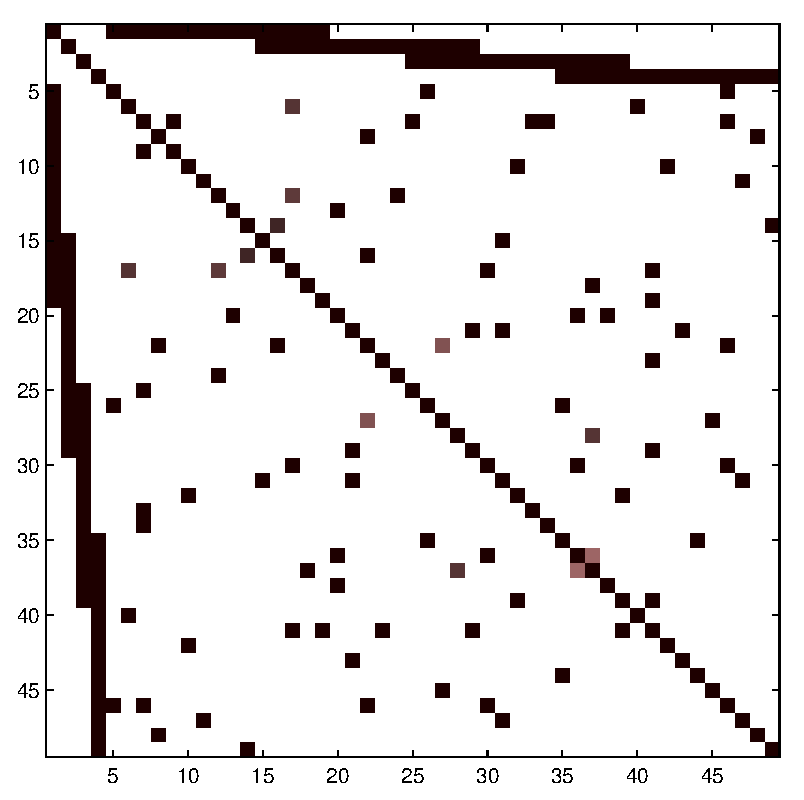
\includegraphics[width=3cm]{fig/overlap_om}}
%\hfill
%\subfigure[Title C]{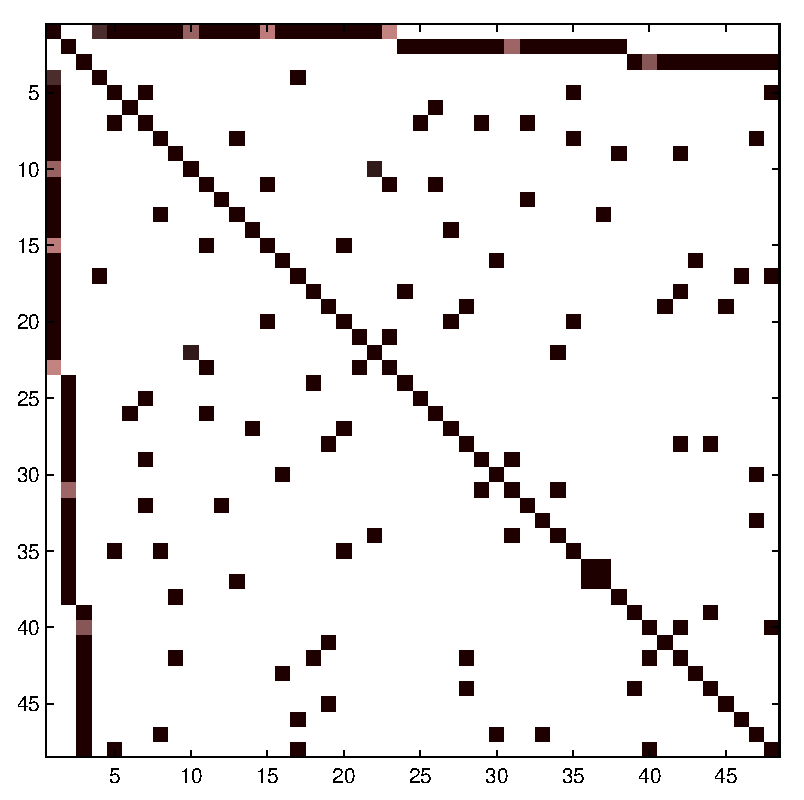
\includegraphics[width=3cm]{fig/diff_om}}
%\hfill
%\\
%\subfigure[Title A]{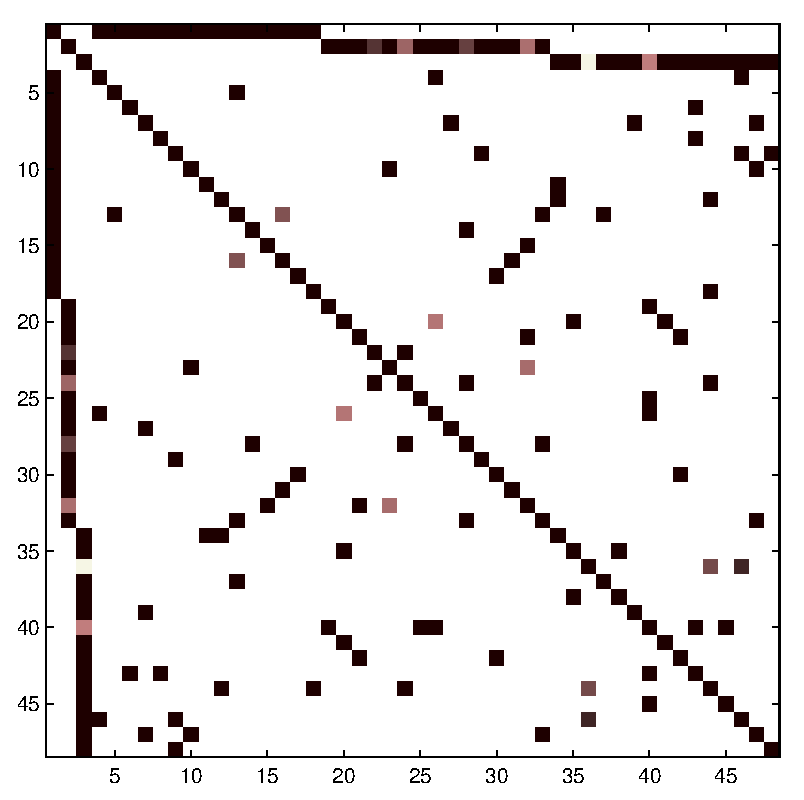
\includegraphics[width=3cm]{fig/disjoint_om}}
%\hfill
%\subfigure[Title B]{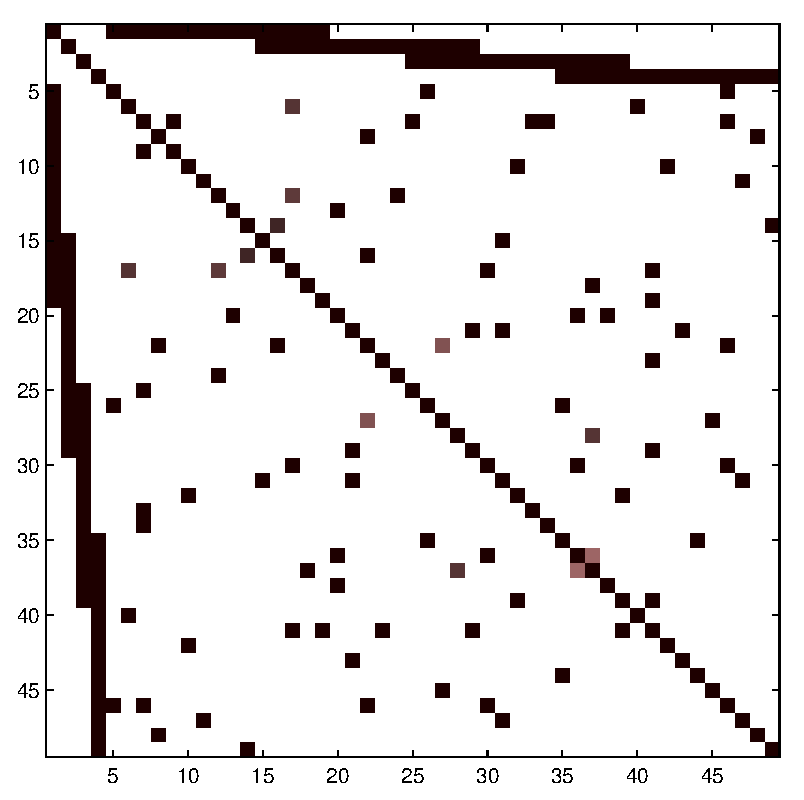
\includegraphics[width=3cm]{fig/overlap_om}}
%\hfill
%\subfigure[Title C]{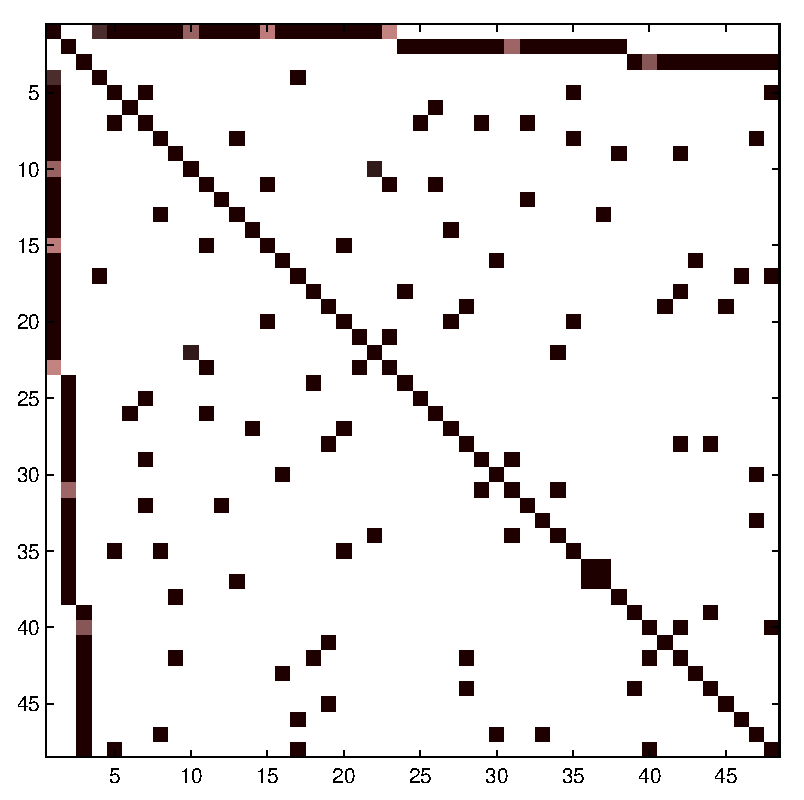
\includegraphics[width=3cm]{fig/diff_om}}
%\hfill
%\caption{Title for both}
%\end{figure}

%\begin{figure}
%\center
%\hfill
%\subfigure[Title A]{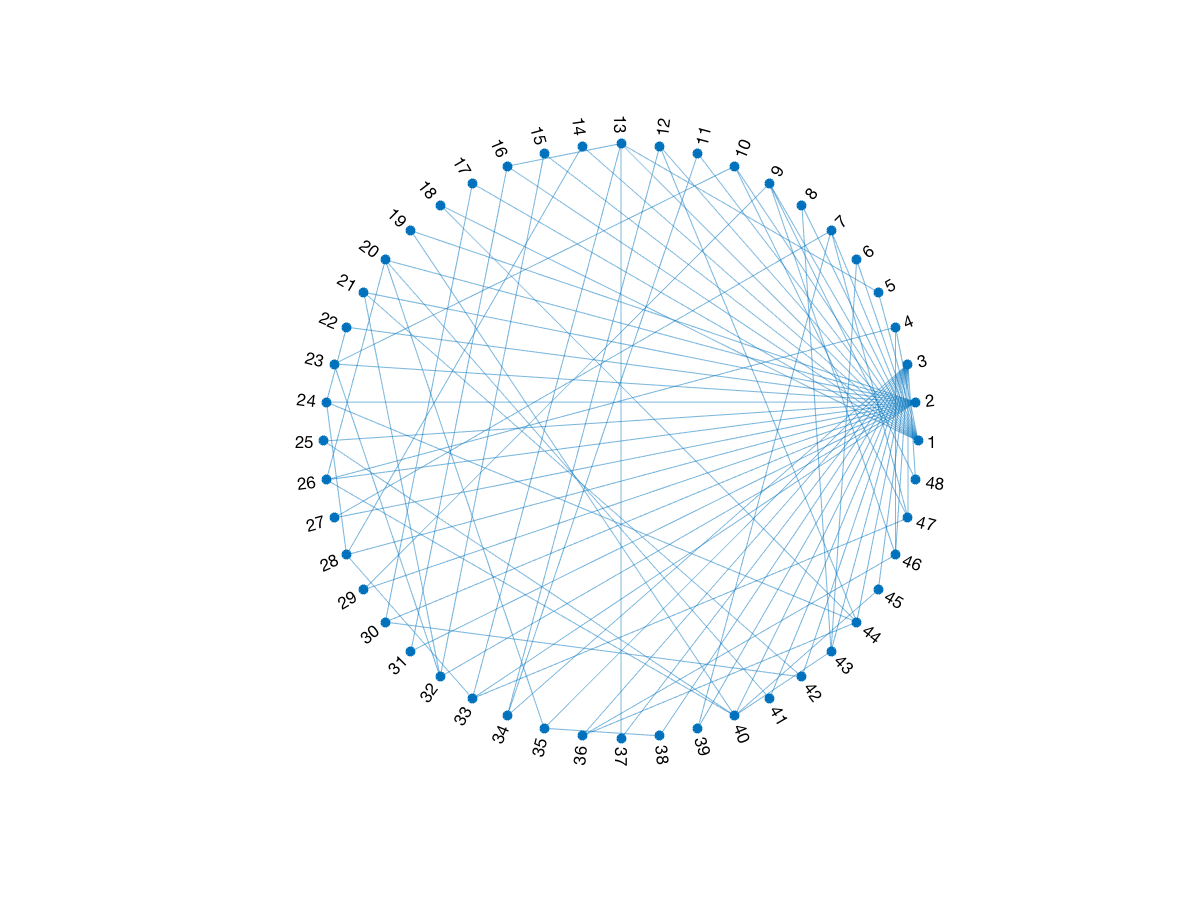
\includegraphics[width=4cm]{fig/disjoint_graph}}
%\hfill
%\subfigure[Title B]{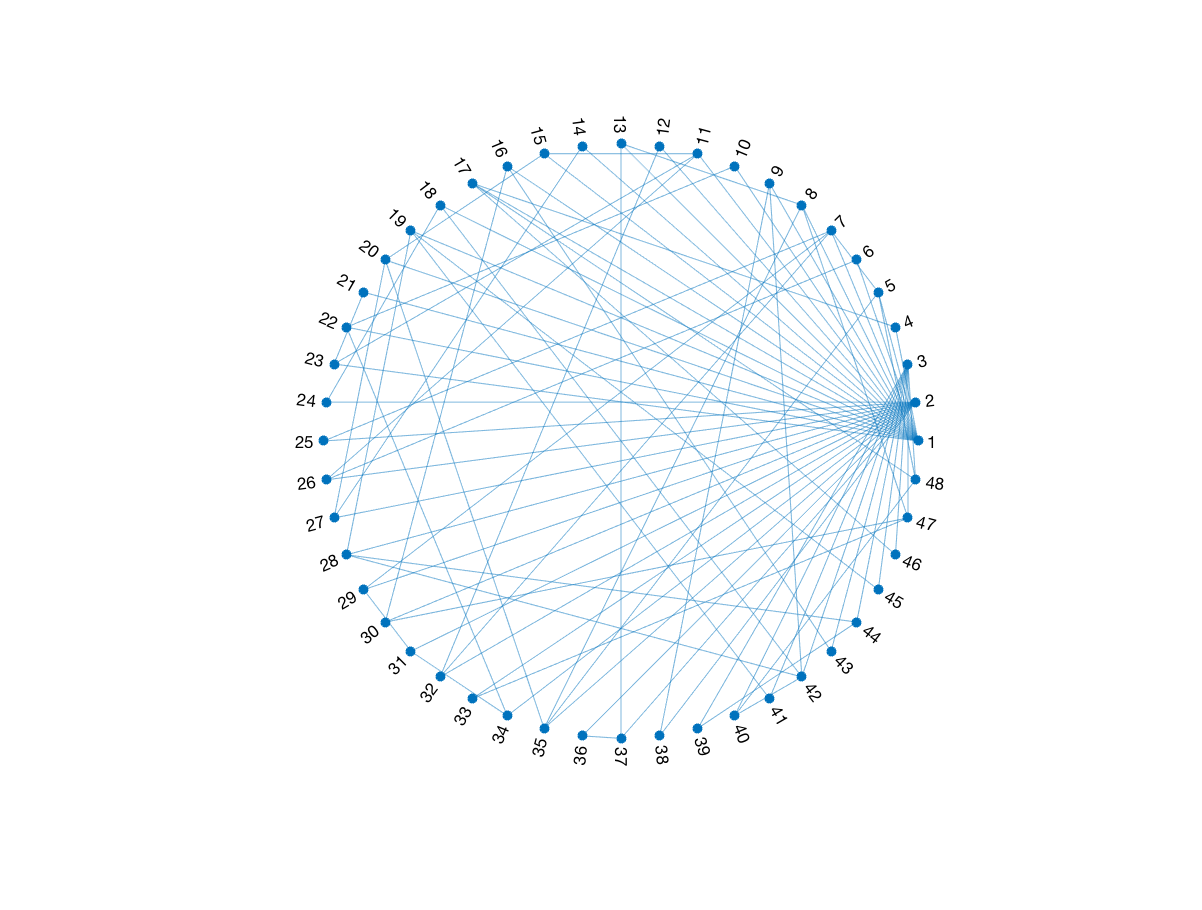
\includegraphics[width=4cm]{fig/diff_graph}}
%\hfill
%\subfigure[Title C]{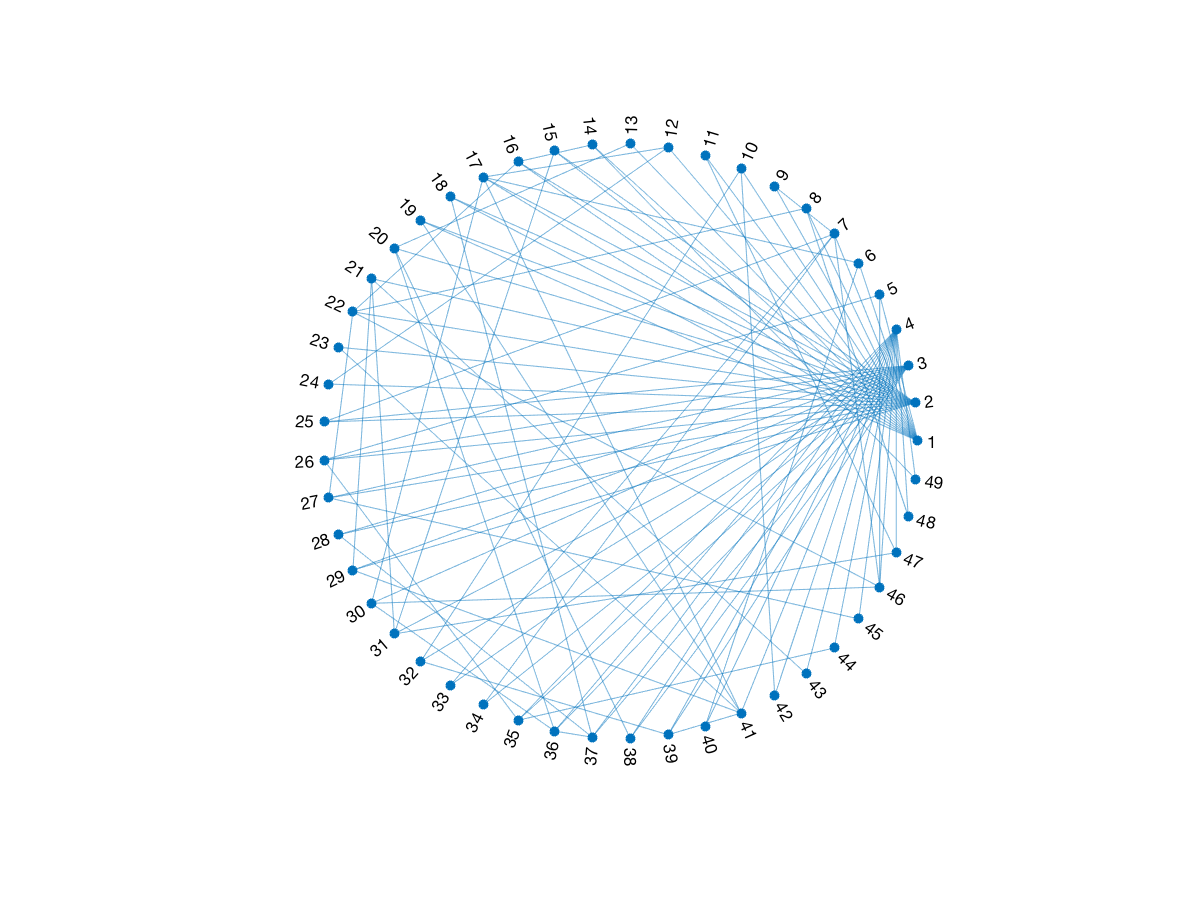
\includegraphics[width=4cm]{fig/over_graph}}
%\caption{Title for both}
%\end{figure}

%\begin{figure}
%\label{fig:synth}
%\center
%\hfill
%\subfigure[ours]{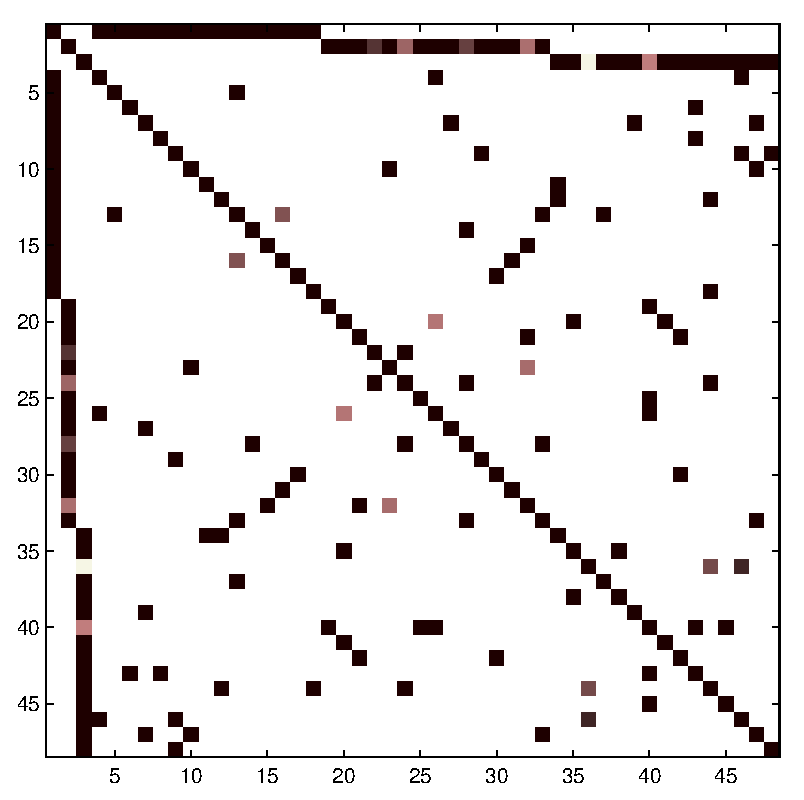
\includegraphics[width=2.2cm]{fig/disjoint_om}}
%\hfill
%\subfigure[$\ell_1+\tr$]{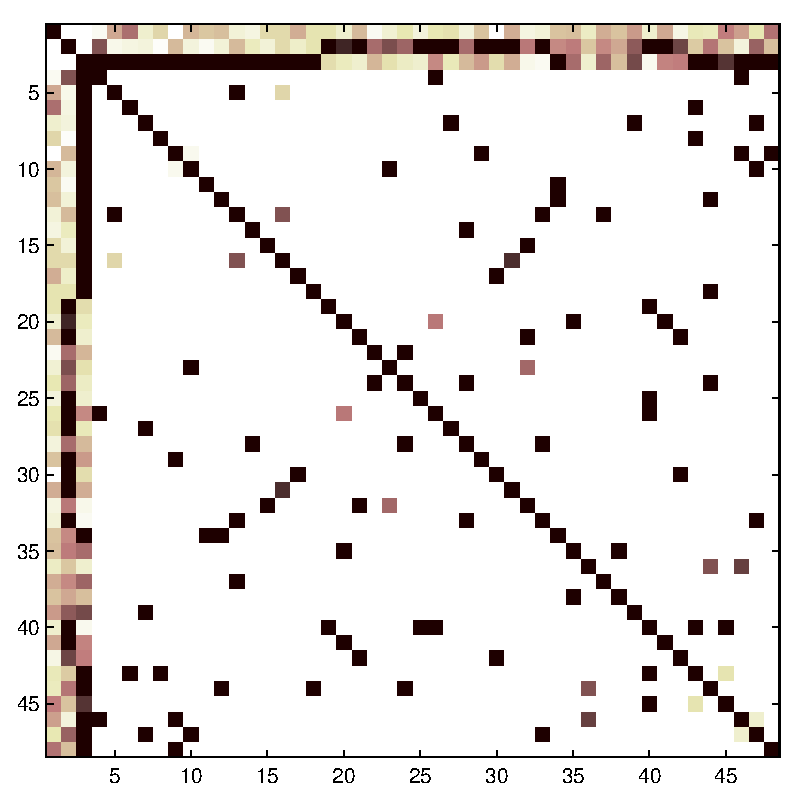
\includegraphics[width=2.2cm]{fig/disjoint_tr}}
%\hfill
%\subfigure[ours]{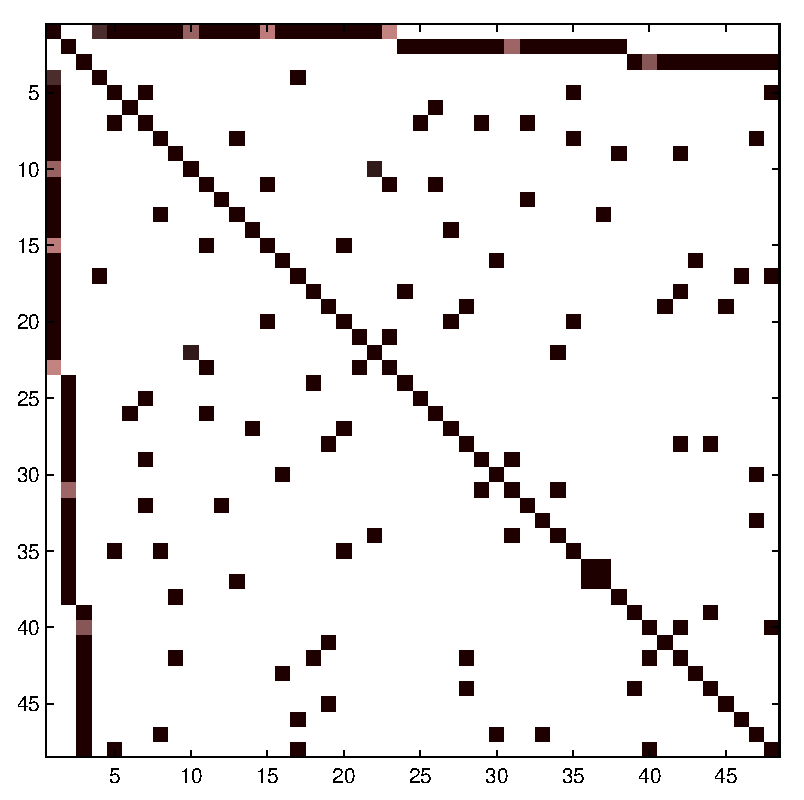
\includegraphics[width=2.2cm]{fig/diff_om}}
%\hfill
%\\
%\subfigure[$\ell_1+\tr$]{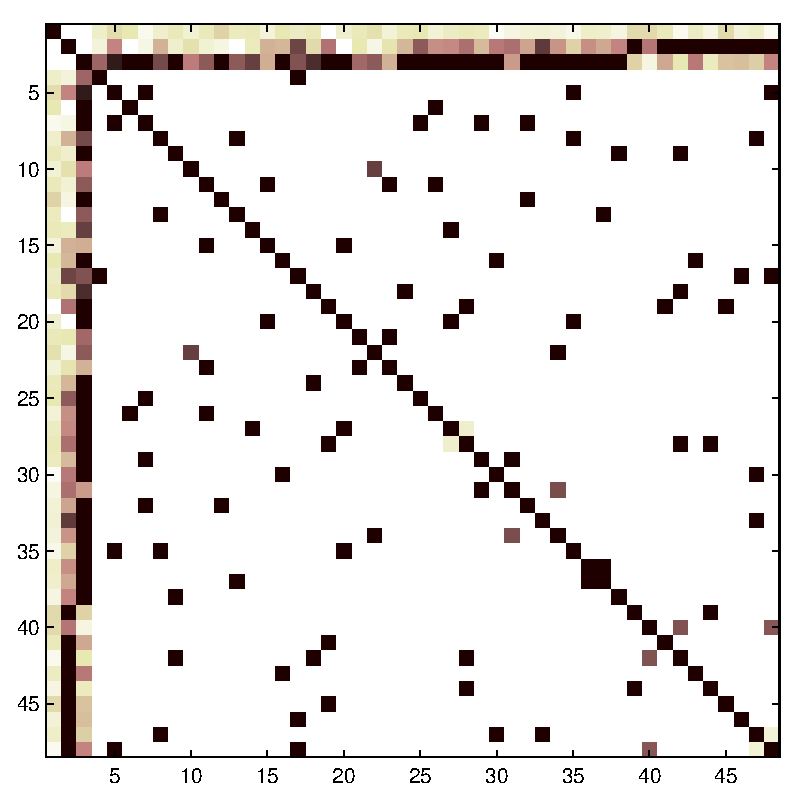
\includegraphics[width=2.2cm]{fig/diff_tr}}
%\hfill
%\subfigure[ours]{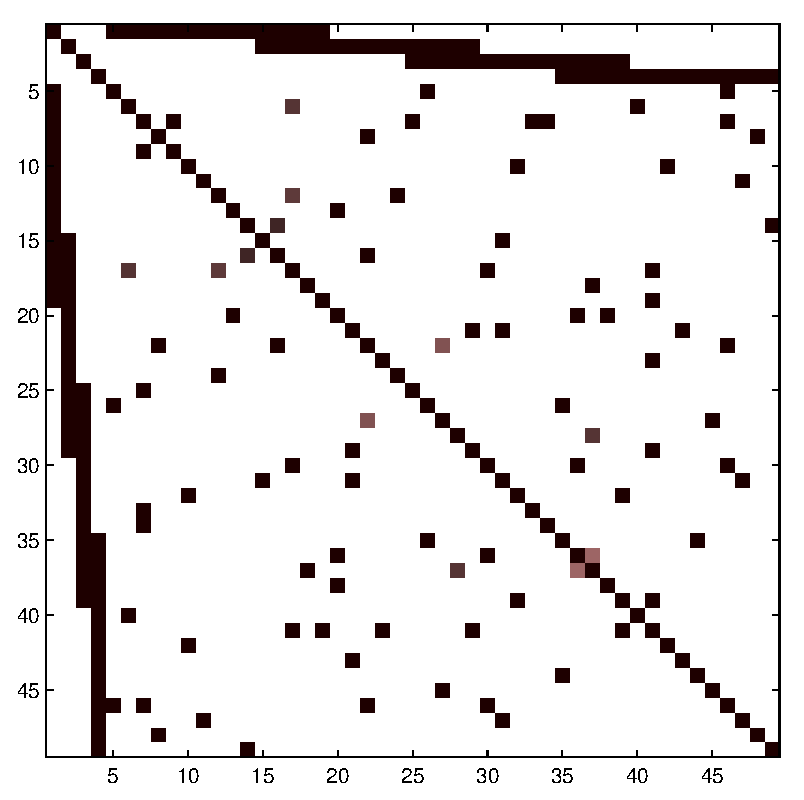
\includegraphics[width=2.2cm]{fig/overlap_om}}
%\hfill
%\subfigure[$\ell_1+\tr$]{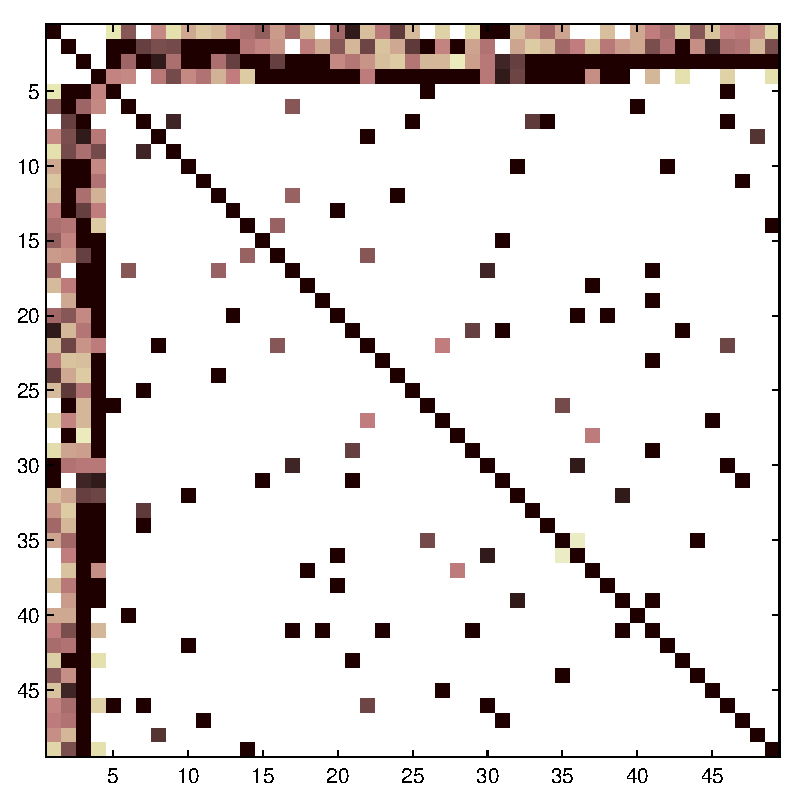
\includegraphics[width=2.2cm]{fig/overlap_tr}}
%\hfill
%\caption{Estimated complete concentration matrices: for \textit{model 1} in (a) ours and (b) $\ell_1+\tr$ regularization; for \textit{model 2} in (c) ours and (d) $\ell_1+\tr$ regularization; for \textit{model 3} in (e) ours and (f) $\ell_1+\tr$ regularization }
%\end{figure}

\begin{figure}
\label{fig:synth}
\center
\begin{tabular}{cc}
    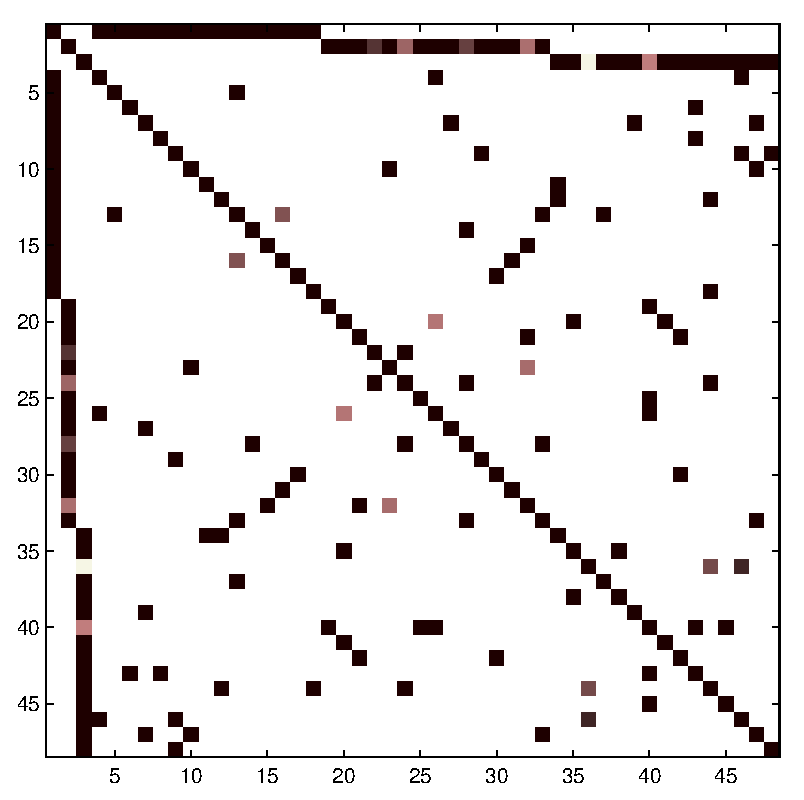
\includegraphics[width=.3\linewidth]{fig/disjoint_om} 
  & 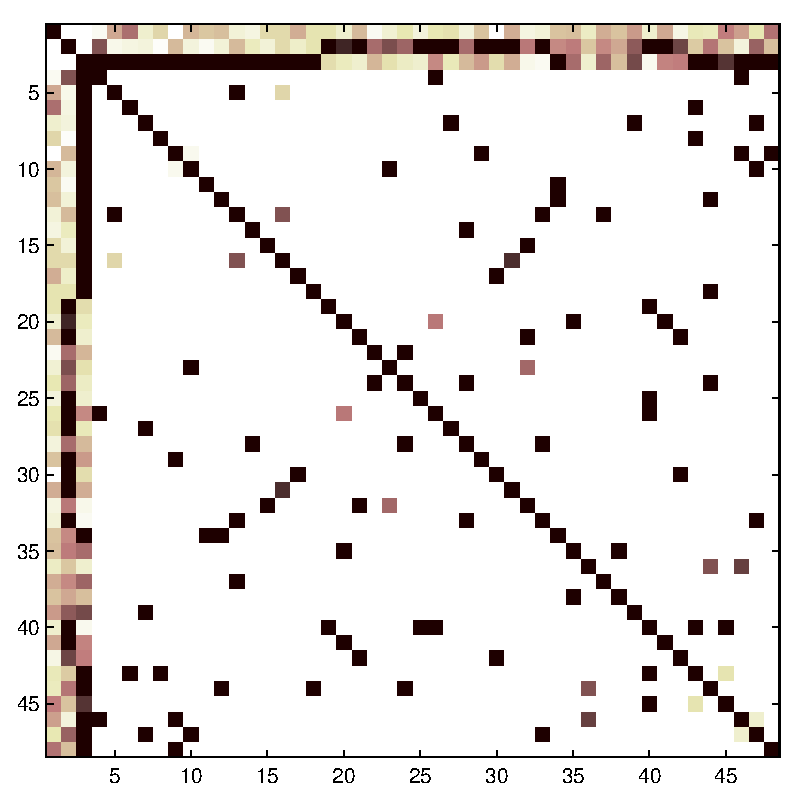
\includegraphics[width=.3\linewidth]{fig/disjoint_tr} 
   \\    (a) \textit{model 1}, ours & (d)  \textit{model 1}, $\ell_1+\tr$ \\[6pt]
      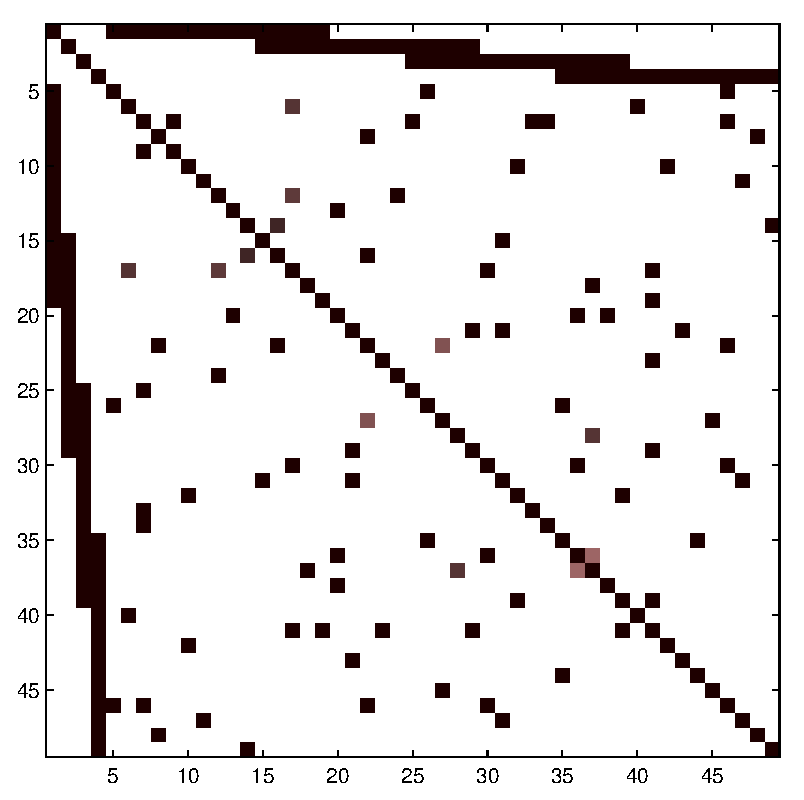
\includegraphics[width=.3\linewidth]{fig/overlap_om}
  &   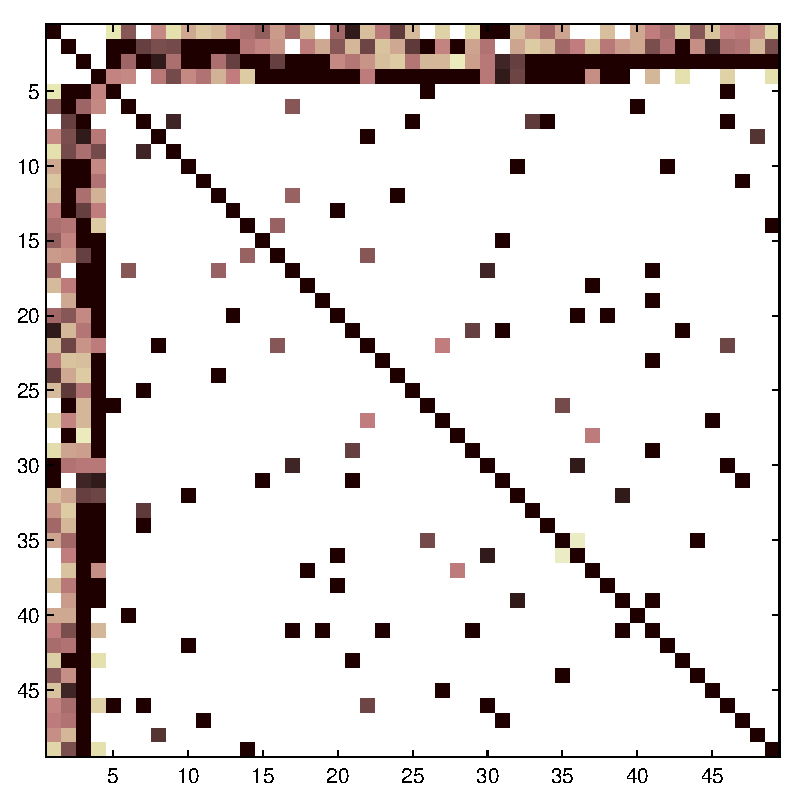
\includegraphics[width=.3\linewidth]{fig/overlap_tr}
   \\    (b)  \textit{model 2}, ours   & (e)  \textit{model 2}, $\ell_1+\tr$    \\[6pt]
      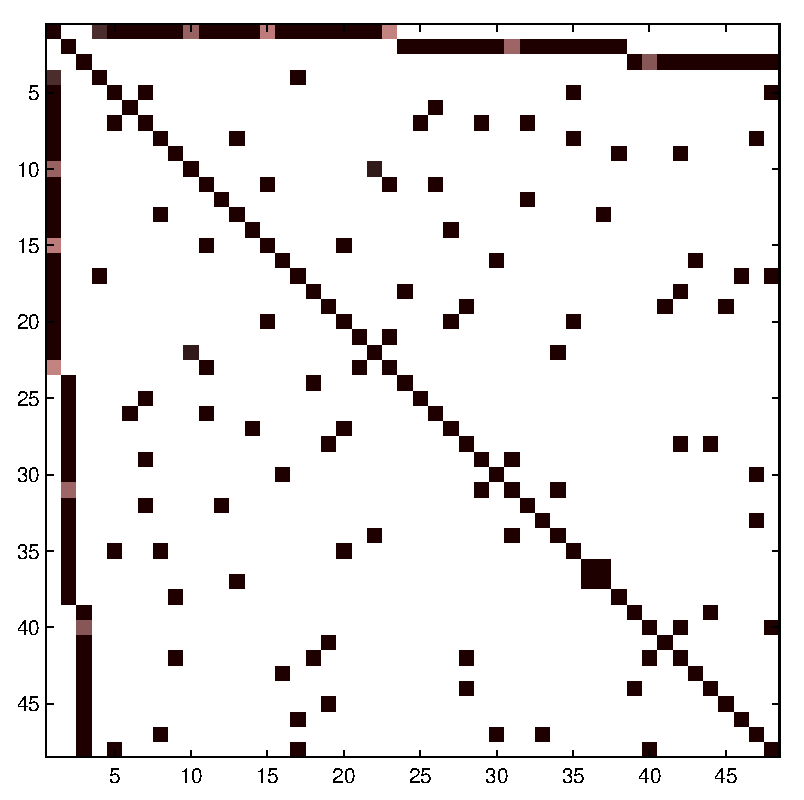
\includegraphics[width=.3\linewidth]{fig/diff_om}
  &   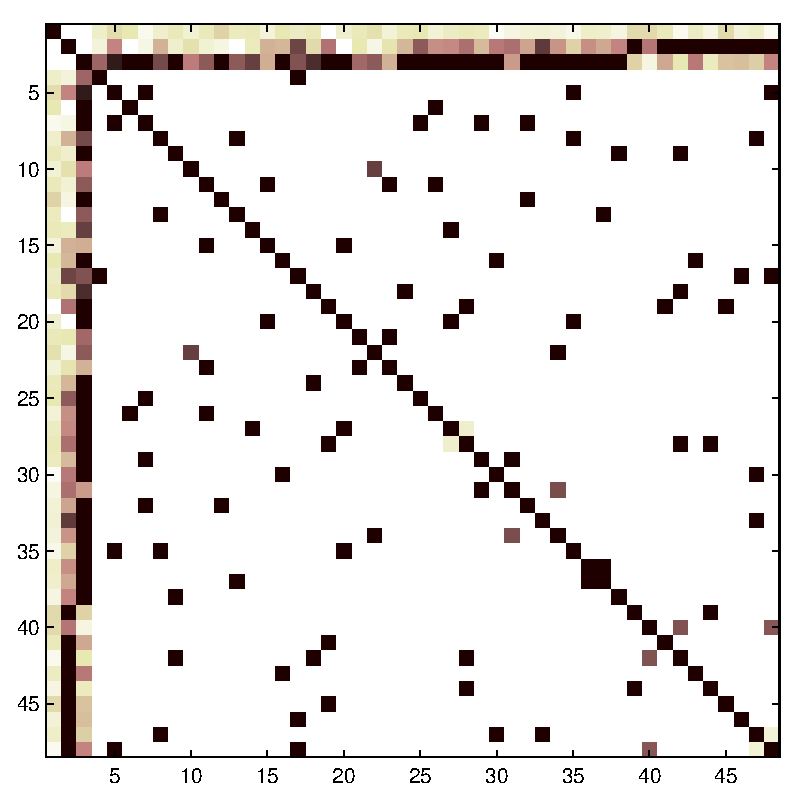
\includegraphics[width=.3\linewidth]{fig/diff_tr}
   \\    (c)  \textit{model 3}, ours & (f)  \textit{model 3}, $\ell_1+\tr$  \\[6pt]
\end{tabular}
\caption{Estimated $|K_{ij}|$, for $K$ the complete concentration matrices where the three (resp. four) first rows and columns correspond to the latent variables of \textit{model 1} and \textit{model 3} (resp. \textit{model 2}) : for \textit{model 1} in (a) ours and (d) $\ell_1+\tr$ regularization; for \textit{model 2} in (b) ours and (e) $\ell_1+\tr$ regularization; for \textit{model 3} in (c) ours and (f) $\ell_1+\tr$ regularization }
\end{figure}

\subsection{Synthetic experiments}

\paragraph{Sparse Wishart matrix}
We describe a protocol to generate a random concentration matrix from a desired graph structure $\mathcal{G}=(V,E)$, where $V$ and $E$ are the set of vertices and edges respectively. We build the incidence matrix of the $B\in\RR^{n\times m}$, where $n$ and $m$ are the numbers of vertices and edges respectively, such that $B_{i,j} = 1$ if the vertex $v_i$ and edge $e_j$ are incident and $0$ otherwise. $\tilde{B}$ is a sparse random matrix with sparsity pattern of $B$ where the nonzeros of $\tilde{B}$ are i.i.d. Gaussian variables. We obtain a random concentration matrix with the imposed structure sparse $K=\tilde{B}\tilde{B}^{\top}$. Note that this procedure is an extension of Wishart matrices to sparse matrices. The obtained matrix $A$ is automatically p.s.d.

In our experiments we choose the latent structure of the graph and we build the sparse structure from an Erd\"os–R\'enyi model, where each edge has a fixed probability $p_{s}=0.01$ of being present or absent, independently of the other edges. We obtain the covariance on observed variables from the Schur complement of the concentration matrix with respect to latent variables as in equation (\ref{schur}). The settings for the experiment are the following : wet set the number of observed variables to $160$. We add $4$ latent variables connected to non overlapping groups of $35$ observed variables and we generate $2000$ samples. Figure \ref{fig:synthlarge} shows the low rank component of the ground truth covariance and the low rank component obtained by our method. We clearly recover the latent structure of the graph, i.e. the four groups of $35$ variables. \\


\begin{figure}
\label{fig:synthlarge}
\center
\begin{tabular}{cc}
    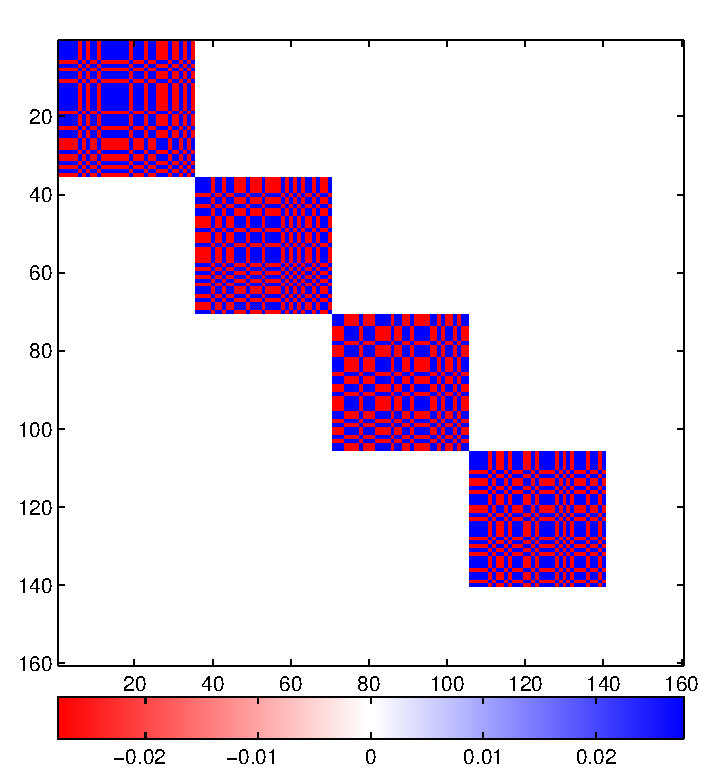
\includegraphics[width=.4\linewidth]{fig/M} 
  & 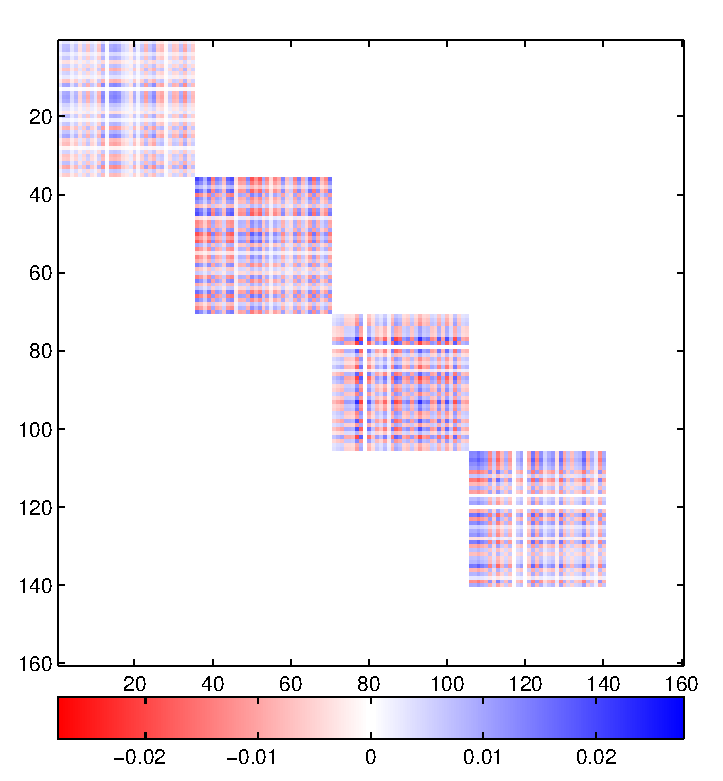
\includegraphics[width=.4\linewidth]{fig/outputM} 
   \\    (a) & (b) \\[6pt]
\end{tabular}
\caption{\TODO{Experiment on bigger model showing blocks $p = 160$,$n= 2000$,$k = 35$}}
\end{figure}

\section{Conclusion}
We consider a family of latent variable Gaussian graphical model whose concentration matrix has a sparse plus low-rank structure. We introduce a regularization to impose more structure on the low rank component, as a sum of multiple low-rank and $k$-sparse factors, and derive a convex formulation. We propose an efficient algorithm to optimize this problem and show promising results for recovering the structure of the complete GGM in the experiments. We provide a first result for identifiability condition. Futurework includes extending the framework to multiple levels of sparsity and generalizing identifiability conditions for recovery guarantees on our optimisation problem .

%\subsubsection*{References}
\bibliographystyle{apalike}
\bibliography{phd}

\end{document}